\documentclass{handoutForSolutions}
%\SetInstructor{name here}
\SetCourseTitle{Yihong Liu}
\SetSemester{Attanasio, Meghir \& Santiago (2011)}
%\SetHandoutTitle{Right top}
%\SetDueDate{\today Right bottom}

\usepackage{MastenAuthor_Environments}
\usepackage{MastenAuthor_Boxes}
\usepackage{MastenShortcuts}
\usepackage{MnSymbol}
\usepackage{amsmath, bm}
\usepackage{float}
\usepackage{ulem}
\normalem



% For manually numbering results
\usepackage{thmtools}
\declaretheoremstyle[notefont=\bfseries,notebraces={}{},%
    headpunct={},postheadspace=1em]{mystyle}
\declaretheorem[style=mystyle,numbered=no,name=Theorem]{theorem_hand_numbered}
\declaretheorem[style=mystyle,numbered=no,name=Lemma]{lemma_hand_numbered}
\declaretheorem[style=mystyle,numbered=no,name=Proposition]{proposition_hand_numbered}
\declaretheorem[style=mystyle,numbered=no,name=Assumption]{assumption_hand_numbered}
\declaretheorem[style=mystyle,numbered=no,name=Corollary]{corollary_hand_numbered}
\declaretheorem[style=mystyle,numbered=no,name=Definition]{definition_hand_numbered}
\declaretheorem[style=mystyle,numbered=no,name=Condition]{condition_hand_numbered}

\newenvironment{theoremboxed_hand_numbered}{\begin{mdframed}\begin{theorem_hand_numbered}}{\end{theorem_hand_numbered}\end{mdframed}}
\newenvironment{lemmaboxed_hand_numbered}{\begin{mdframed}\begin{lemma_hand_numbered}}{\end{lemma_hand_numbered}\end{mdframed}}
\newenvironment{propositionboxed_hand_numbered}{\begin{mdframed}\begin{proposition_hand_numbered}}{\end{proposition_hand_numbered}\end{mdframed}}
\newenvironment{corollaryboxed_hand_numbered}{\begin{mdframed}\begin{corollary_hand_numbered}}{\end{corollary_hand_numbered}\end{mdframed}}



\begin{document}


\begin{center}
{ \normalfont \Large \textbf{Education Choices in Mexico:
Using a Structural Model and a Randomized Experiment to Evaluate PROGRESA} }
\end{center}

\section{INTRODUCTION}
In 1998, the Mexican government started a remarkable new program in rural localities. PROGRESA was one of the first and probably the most visible of a new generation of interventions, whose main aim is to improve the process of human capital accumulation in the poorest communities by providing cash transfers conditional on specific types of behaviour in three key areas targeted by the program: nutrition, health, and education. Arguably the largest of the three components of the program was the education. Mothers in the poorest households in a set of targeted villages are given grants to keep their children in school. In the first version of the program, which has since evolved and is now called Oportunidades, the grants started in third grade and increased until the ninth and were conditional on school enrolment and at- tendance. PROGRESA was noticeable and remarkable not only for the original design but also because, when the program begun, the Mexican government started a rigorous evaluation of its effects.

The evaluation of PROGRESA is greatly helped by the existence of a high-quality data set whose collection was started at the outset of the program, between 1997 and 1998. The PRO- GRESA administration identified 506 communities that qualified for the program and started the collection of a rich longitudinal data set in these communities. Moreover, 186 of these com- munities were randomized out of the program with the purpose of providing a control group that would enhance the evaluation. However, rather than being excluded from the program all together, in the control villages the program was postponed for about 2 years, during which period, four waves of the panel were collected. Within each community in the evaluation sam- ple, all households, both beneficiaries (i.e. the poorest) and non-beneficiaries, were covered by the survey. In the control villages, it is possible to identify the would-be beneficiaries were the program to be implemented.

A better understanding of the effectiveness of policies that promote school attendance is important:$\footnote{For an evaluation of an equivalent program in a high income country see Dearden et al. (2009).}$ deficits in the accumulation of human capital have been identified by several commentators as one of the main reasons for the relatively modest growth performance of Latin American economies in comparison, for instance, with some of the South East Asian countries (see, for instance, Behrman, Duryea and Székely, 1999; Behrman and Todd, 1999, 2000). For this reason, the program we study and similar ones have received considerable attention in Latin America.

By all accounts and evidence, the evaluation of PROGRESA, based on the large randomized experiment described above, was highly successful (see Schultz, 2004). Given the evaluation design, the program impacts could be estimated by comparing mean outcomes between treatment and control villages. These estimates, on their own, can answer only a limited question (albeit without relying on any parametric or functional form assumption), namely how did the specific program implemented in the experiment affect the outcomes of interest. However, policy may require answers to much more refined questions, such as extrapolating to different groups or altering the parameters of the initial program.

The aim of this paper is to analyse the impact of monetary incentives on education choices in rural Mexico, to discuss effective design of interventions aimed at increasing school enrolment of poor children, and to illustrate the benefits of combining randomized experiments with structural models. To achieve these goals, we estimate a simple structural model of education choices using the data from the PROGRESA randomized experiment. We then use the model to simulate the effect of changes to some of the parameters of the program.

PROGRESA effectively changes the relative price of education and child labour in a controlled and exogenous fashion. A tightly parameterized model, under suitable restrictions (see below), could identify the effect of the program even before its implementation, using variation in the opportunity cost of schooling (i.e. the wage) across communities where the program is not available. This is the strategy followed, in a recent paper, by Todd and Wolpin (2006) (TW henceforth). They identify the impact of the program from variation in child wages across villages in which the program is not implemented and estimate their model without using the variability induced by the PROGRESA. Their approach does not require experimental variation other than as a validation for their model.

Like TW, we estimate a structural model, but our approach and objectives are different. We use both treatment and control villages exploiting the variation in the grant induced by the randomized experiment to estimate a specification that could not be estimated without the program: critically, the marginal utility of the grant is different from the marginal utility of any other source of income; we illustrate this point with a simple model in Section 4.1 and we show that it has important implications for the impact of the program.

There are many reasons why the grant might have a different marginal utility than other source of income such as the wage; these relate to the structure of preferences, the nature of within-household decision making, and the perception of the grant. In some cases, such effects can only be taken into account using the variation in a school grant such as that induced by the experiment. This is specifically the case when income pooling fails within the household.$\footnote{For tests of income pooling, see among others Thomas (1990) or Blundell {\it et} $aT$ (2007).}$

Thus, the use of non-experimental data to carry out ex ante evaluation, with no variation in school grants, requires additional assumptions: one needs to assume that conditional on the activity of the child (education or work), the income of the child and other household income have the same effect on utility. This assumption allows one to aggregate other household and child income into one single pooled income measure as TW do. A violation of such an assumption may relate to preferences or within-household allocations. For example, while the PROGRESA grant is always handed over to the mother, income from child labour may be under the control of the father or even of the child if he/she is older. In all these cases, a peso of child income from work is different from a peso of child income from a school grants programme and both are potentially different from a peso of income from other sources. At least in the context of this population, our results clearly indicate that such differences are crucially important.

Does this mean that ex ante evaluation is infeasible in this context? This would be a rash conclusion because there may well be suitable observational data that could help resolve the issues we raise, e.g. data from a population where some children receive scholarships of varying amounts: given suitable exogeneity assumptions, in this case there would be income attached to attending schooling and the necessary variation to identify its effects; this is not the case in the PROGRESA sample of controls. But even if such variation exists in the data, experimen- tal information can clearly be important for understanding behaviour, if anything because the variation induced by the experiment is guaranteed to be exogenous. Thus, one can think of using experimental variation and indeed designing experiments to generate such variability so as to es- timate more credibly structural models capable of richer policy analysis. In this sense, our work draws from the tradition of Orcutt and Orcutt (1968), who advocate precisely this approach, which found an early expression in the work based on the negative income tax experiments, such as in Burtless and Hausman (1978) and Moffitt (1979). The general point we make is that the experimental variation can help identify economic effects under more general conditions than the observational data, while the structural model can help provide an interpretation of the experimental results and broaden the usefulness of the experiment.

The fact that we estimate a model that, in some dimensions, is more general than the one by TW and that requires the explicit use of the experimental variation to be identified is not the only difference between the two papers. Our approach considers explicitly and estimates the general equilibrium (GE) effects that the program might have on the wages of young children. As mentioned above, PROGRESA was randomized across localities rather than across house- holds. As these localities are isolated from each other, this experimental design also affords the possibility of estimating general equilibrium effect induced by the program. Although some papers in the literature (see, for instance, Angelucci and DeGiorgi, 2009) have looked at the im- pact of PROGRSA on prices and other village-level variables, perhaps surprisingly, no study has considered, as far as we know, the effect that the program has had on children wages. One could imagine that, ifthe program is effective in increasing school participation, a reduction in the supply of child labour could result in an increase in child wages which, in turn, would result in an attenuation ofthe program's impact. Here, we estimate this impact (taking into account the fact that child wages are observed only for the selected subset of children who actually work) and establish that the program led to an increase in these wages in the treatment municipalities by decreasing the labour supply of children. We incorporate these GE impacts within our model and in our simulations.

Finally, there are also differences in the estimation approach, as well as in the specification of the models, between this paper and that of TW. Both our model and TW’s include the presence of habits in the utility from schooling. This creates an initial condition problem in the estimation of the structural model. While TW tackle this issue by functional form assumptions and the implied non-linearities, we also exploit the increasing availability of schooling as an instrument to control for the initial condition problem so as to better disentangle state dependence from unobserved heterogeneity. As for the specification, TW’s model solves a family decision problem, including trade-offs between children and fertility, which we do not. Considering fertility effects is potentially interesting. However, it should be pointed out that the programme did not have any effects on fertility.$\footnote{TW's model of fertility is identified only using the observed cross-sectional variation which may not necessarily reflect exogenous differences in incentives.}$ What has informed our modelling choices is the focus on using the incentives introduced by the programme in some localities to identify in a credible fashion our education choice model.

The rest of the paper is organized as follows. In Section 2, we present the main features of the program and of the evaluation survey we use. In Section 3, we present some simple results on the effectiveness of the program based on the comparison of treatment and control villages. In Section 4, we present a structural dynamic model of education choices and describe its various components. Section 5 briefly discusses the estimation of the model. Section 6 presents the results we obtain from the estimation of our model. We also report the results of a version of the model that imposes some restrictions that approximate the model estimated by TW. Section 7 uses the model to perform a number of policy simulations that could help to fine-tune the pro- gram. Finally, Section 8 concludes the paper with some thoughts about open issues and future research.




\newpage


\section{THE PROGRSA PROGRAM}
PROGRESA was started in 1997 by the Zedillo administration. The program introduced a number of incentives and conditions with which participant households had to comply to keep receiving the program’s benefits. At the same time, the administration put in place a quantitative evaluation of the program’s impact based on a randomized design:
\subsection{The specifics of the PROGRESA program}
PROGRESA is the Spanish acronym for “Health, Nutrition and Education” , that are the three main areas of the program. PROGRESA is one of the first and probably the best known of the so-called “conditional cash transfers,” which aim at alleviating poverty in the short run while at the same time fostering the accumulation of human capital to reduce it in the long run. This is achieved by transferring cash to poor households under the condition that they engage in behaviours that are consistent with the accumulation of human capital: the nutritional subsidy is paid to mothers who register the children for growth and development check-ups and vaccinate them as well as attend courses on hygiene, nutrition, and contraception. The education grants are paid to mothers if their school-age children attend school regularly.

The program has received considerable attention and publicity. More recently, programs similar to and inspired by PROGRESA have been implemented in Colombia, Honduras, Nicaragua, Argentina, Brazil, Turkey, and other countries. Rawlings (2004) contains a survey of some of these programs. Skoufias (2001) provides additional details on PROGRESA and its evaluation.

PROGRESA is first targeted at the locality level. The program was then targeted within each community by proxy means testing. Individual households in a targeted community could qualify or not for the program depending on a single indicator, the first principal component of a number of variables (such as income, house type, presence of running water, and so on). Eligibility was determined in two steps. First, a general census of the PROGRESA localities measured the variables needed to compute the indicator and each household was defined as “poor” or “not-poor” (where “poor” is equivalent to eligibility). Subsequently, in March 1998, an additional survey was carried out and some households were added to the list of beneficiaries. This second set of beneficiary households are called “densificados”. Fortunately, the reclassification survey was operated in both treatment and control towns.

The largest component of the program is the education. Beneficiary households with school- age children receive grants conditional on school attendance. The size of the grant increases with the grade and, for secondary education, is slightly higher for girls than for boys. In Table 1, we report the grant structure. All the figures are in current pesos and can be converted to U.S. dollars at approximately an exchange rate of 10 pesos per dollar. In addition to the (bi)monthly payments, beneficiaries with children in school age receive a small annual grant for school supplies.
\begin{figure}[H]
\centering
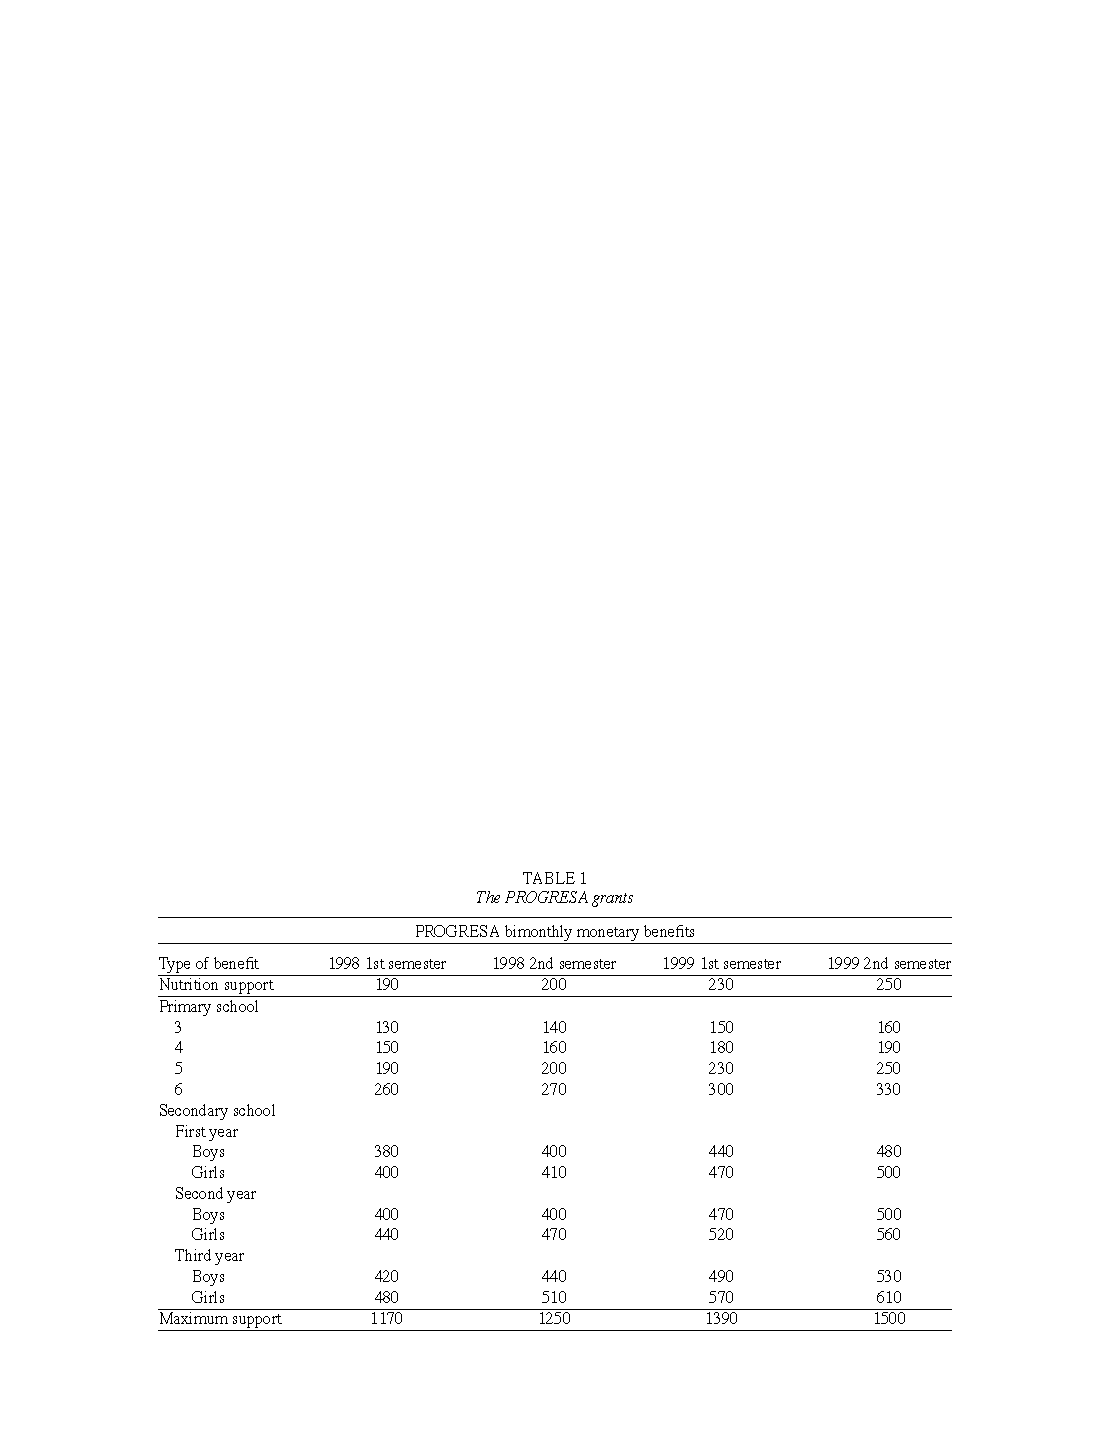
\includegraphics[width=1\linewidth]{image/AttanasioMeghir Santiago2011Figure1.pdf}
\end{figure}
For logistic and budgetary reasons, the program was phased in slowly but is currently very large. In 1998, it was started in less than 10,000 localities. However, at the end of 1999, it was implemented in more than 50,000 localities and had a budget of about US\$777 million or 0.2\% of Mexican gross domestic product (GDP). At that time, about 2.6 million households, or 40\% of all rural families and one-ninth of all households in Mexico, were included in the program. Subsequently, the program was further expanded and, in 2002–2003 was extended to some urban areas.

The program represents a substantial help for the beneficiaries. The nutritional component of 100 pesos per month (or 10 US\$10) in the second semester of 1998 corresponded to 8\% of the beneficiaries’ income in the evaluation sample.

As mentioned above, the education grants are conditional to school enrolment and attendance of children and can be cumulated within a household up to a maximum of 625 pesos (or 62.5 dollars) per month per household or 52\% of the average beneficiary’s income. The average grant per household in the sample we use was 348 pesos per month for households with children and 250 for all beneficiaries or 21\% of the beneficiaries income. To keep the grant, children have to attend at least 85\% of classes. Upon not passing a grade, a child is still entitled to the grant for the same grade. However, if the child fails the grade again, it looses eligibility.



\subsection{The evaluation sample}
Before starting the program, the agency running it decided to start the collection of a large data set to evaluate its effectiveness. Among the targeted localities, 506, located in 7 of the 31 Mexican states, were chosen randomly and included in the evaluation sample. The 1997 survey was supplemented, in March 1998, by a richer survey in these villages. All households in these villages were interviewed, for a total of roughly 25,000 households. Using the information of the 1997 survey and that of the March 1998 survey, each household can be classified as poor or non-poor, i.e., each household can be identified as being entitled or not to the program.

As mentioned above, in 320 of the 506 localities included in the evaluation sample the program was started immediately, i.e. in May 1998, while in the remaining 186, it was started almost 2 years later. The 320 “treatment localities” were chosen randomly.

An extensive survey was carried out in the evaluation sample: after the initial data collection between the end of 1997 and the beginning of 1998, an additional four instruments were collected in November 1998, March 1999, November 1999, and April 2000. Within each village in the evaluation sample, the survey covers all the households and collects extensive information on consumption, income, transfers, and a variety of other variables. For each household member, including each child, there is information about age, gender, education, current labour supply, earnings, school enrolment, and health status. The household survey is supplemented by a locality questionnaire that provides information on prices of various commodities, average agricultural wages (both for males and females), as well as institutions present in the village and distance of the village from the closest primary and secondary school (in kilometers and minutes).

At the time of the 1997 survey, each household in the treatment and control villages was defined as either eligible or non-eligible. Subsequently, in March 1998 before the start of the program, some of the non-eligible household were reclassified as eligible. However, a considerable fraction of the newly eligible households, due to administrative delays, did not start receiving the program until much later. In some of the results we present below, we distinguish these households. In the estimation of the structural model, we consider as beneficiary a household that actually receives the program.
\newpage


\section{MEASURING THE IMPACT OF THE PROGRAM: TREATMENT VS. CONTROL VILLAGES}
\subsection{Identification}
As PROGRESA was assigned randomly between treatment and control villages during the expansion phase of the program, it is straightforward to use the evaluation sample to estimate the impact of the conditional cash transfers on school enrolment. Randomization implies that control and treatment samples are statistically identical and estimates of program impacts can be obtained by a simple comparison of means. However, such an exercise estimates the impact of the program as a whole, without specifying the mechanisms through which it operates.

The availability of baseline, pre-program data allows one to check whether the evaluation sample is balanced between treatment and control groups both in terms of pre-program outcomes and in terms of other observable background characteristics. This exercise was performed by Behrman and Todd (1999), who explored a wide range of variables at baseline. The data include information on programme eligibility for both treatment and control villages at baseline. This allows us to make the comparisons separately for eligible and non-eligible households. Behrman and Todd (1999) indicate that, by and large, the treatment and control samples are very well balanced. However, there seem to be some pre-program differences in school enrolment among non-eligible households. While it is not clear why such a difference arises, it might be important to control for these initial differences when estimating impacts.

In this section, we present some estimates of the impact of PROGRESA on school enrolment. These impacts have been widely studied: IFPRI (2002) summarizes the estimates of program impacts on a wide set of outcomes, reported in several studies commissioned within the evaluation of the program. Schultz (2004) presents a complete set of results on the impact of the program on school enrolment, which are substantially similar to those presented here. Here, our focus is on some aspects of the data that are pertinent to our model and to the sample we use to estimate it. And more importantly, by describing the impacts of the program in the sample we use to estimate our structural model, we set the mark against which it will be fitted.

As our structural model will be estimated on boys, we report only the results for them. The effects for girls are slightly higher but not substantially different from those reported here for boys. As we will be interested in how the effect of the grant varies with age, we also report the results for different age groups, although when we consider individual ages, some of the estimates are quite imprecise.

In Table 2, we report the estimated impact for the boys of each age obtained comparing treatment and control villages in October 1998. In the last two rows, we also report the average impacts on boys aged 12–15 years (which is an age group on which TW focus) and on boys aged 10–16 years, that is our entire sample. In the first column of the table, we report enrolment rates among eligible (as of 1997) boys in control villages. In the second column, we show the estimated impacts obtained for boys from households that were declared eligible in 1997 (poor 97). In the third column, we report the results for the boys in all eligible households, including those reclassified in March 1998. Finally, in the fourth column, we report the impacts on the non-eligible children.

The experimental impacts show that the effect of the PROGRESA program on enrolment has a marked inverted U-shape. The program impact is small and not significantly different from zero at age 10. It increases considerably past age 10 to peak at age 14, where our point estimates indicate an impact of 14 percentage points on boys whose households were classified as eligible in 1997. The impact then declines for higher ages, probably a consequence of the fact that the grant was not available, in the first version of the program, past grade 9. The average impact for the boys in our sample (aged 10–16 years) is about 5 percentage points, while for the boys aged 12–15 years is, on average, as high as 6.6\%.

The impact on the households classified as poor in 1997 is slightly higher than on all eligible households, probably a reflection that the impact might be higher for poorer families and the fact that some of the families that were reclassified as eligible in March 1998 (after being classified as non-eligible in 1997) did not receive the program immediately, due to administrative difficulties. A surprising feature of Table 2 is the measured impact on non-eligible children. Although noisy, the estimates for some age groups indicate a large impact on non-eligible boys. Indeed, for the age group 10-16, the effect is even larger than for the eligible children, at almost 8\%. While one could think of the possibility of spillover effects that would generate positive effects on non-eligible children, the size of the impacts we measure in Table 2 is such that this type of explanation is implausible. As we mentioned above, however, if one compares school enrolment rates in 1997 between treatment and control villages, one finds that, among non- eligible households, they are significantly higher (statistically and substantially) in treatment villages than in control villages. This is particularly so for children aged 12-16 years. Instead, enrolment rates in 1997 among eligible children are statistically identical in treatment and control villages. It is therefore possible that the observed difference in enrolment rates among non-eligible households is driven by pre-existing differences between treatment and control towns.

The reason for the difference in enrolment rates among boys (and girls) in non-eligible households between treatment and control villages is not clear. Within our structural model, we account for it by considering one specification that incorporates an unobserved cost component for non-eligible households in control villages. As for measuring the effect of the program as in Table 2, one can use the 1997 data to obtain a difference in difference estimates of its impacts. We report the results of such an exercise in Table Al in the appendix. In this table, the pattern of the impacts among eligible children is largely unaffected (as to be expected given the lack of significant differences between treatment and control villages at baseline for these children). The impacts on the non-eligible children, however, become insignificant. This evidence justifies the interpretation of the evidence in the last column of Table 2 as being caused by pre-existing unobservable differences for non eligible children and justifies our use of a ``non-eligible control'' dummy in our empirical specification.


\newpage

\section{THE MODEL}
We use a simple dynamic school participation model. Each child (or his/her parents) decide whether to attend school or to work taking into account the economic incentives involved with such choices. Parents are assumed here to act in the best interest of the child and consequently we do not admit any interactions between children. We assume that children have the possibility of going to school up to age 17. All formal schooling ends Uy that time. In the data, almost no individuals above age 17 are in school. We assume that children who go to school do not work and vice versa. We also assume that children necessarily choose one of these two options. If they decide to work, they receive a village $/\mathrm{e}\mathrm{d}\mathrm{u}\mathrm{c}\mathrm{a}\mathrm{t}\mathrm{i}\mathrm{o}\mathrm{n}/\mathrm{a}\mathrm{g}\mathrm{e}$ specific wage. If they go to school, they in- cur $\mathrm{a}$ (utility) cost (which might depend on various observable and unobservable characteristics) and, with a certain probability, progress a grade. At 18, everybody ends formal schooling and reaps the value of schooling investments in the form of a terminal value function that depends on the highest grade passed. The PROGRSA grant is easily introduced as an additional monetary reward to schooling that would be compared to that of working.

The model we consider is dynamic for two main reasons. First, the fact that one cannot attend regular school past age 17 means that going to school now provides the option of completing some grades in the future: $i.e$. a 6-year-old child who wants to complete secondary education has to go to school (and pass the grade) every single year, starting from the current. This source 
\begin{figure}[H]
\centering
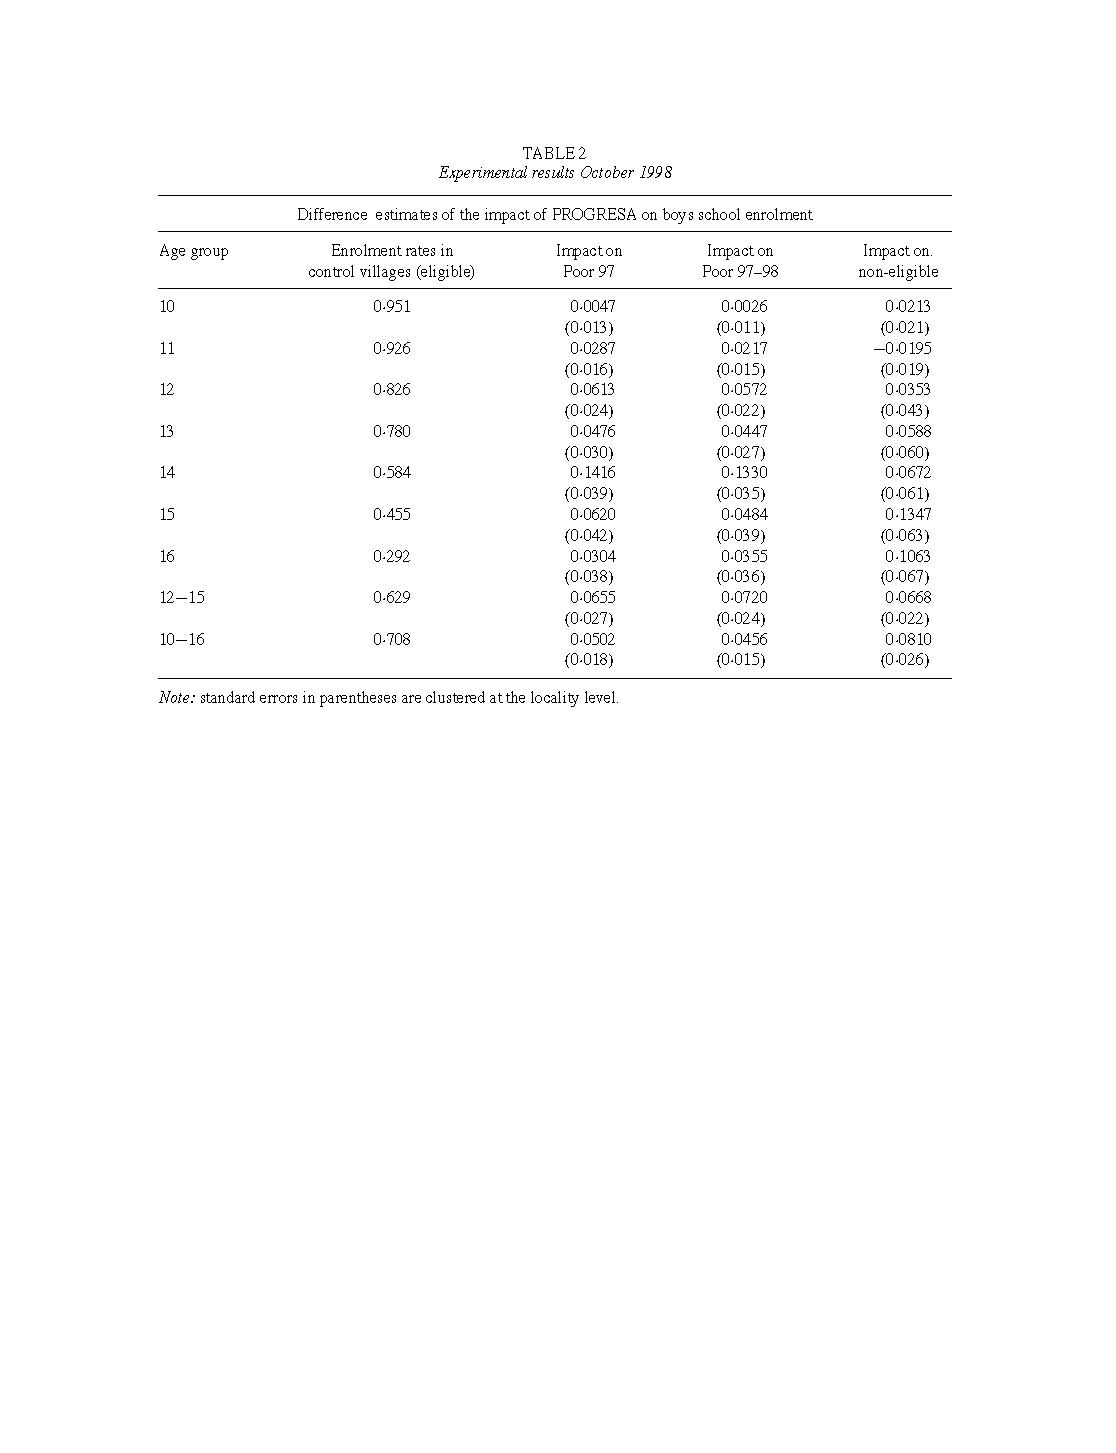
\includegraphics[width=1\linewidth]{image/AttanasioMeghir Santiago2011Figure2.pdf}
\end{figure}
of dynamics becomes particularly important when we consider the impact of the PROGRSA grants since children, as we saw above, are only eligible for six grades: the last 3 years of primary school and the first 3 years of secondary. Going through primary school (by age 14), therefore, also ``buys'' eligibility for the secondary school grants. Second, we allow for state dependence: the number of years of schooling affects the utility of attending in this period. We explicitly address the initial condition problem that arises from such a consideration and discuss the related identification issues at length below. State dependence is important because it may be a mechanism that reinforces the effect of the grant.

Before discussing the details of the model, it is worth mentioning that using a structural approach allows us to address the issue of anticipation effects and the assumptions required for their identification. PROGRSA as well as other randomized experiments or pilot studies create a control group by delaying the implementation of the program in some areas rather than excluding them completely. It is therefore possible that the control villages react to the program prior to its implementation, depending on the degree to which they believe they will eventually receive it. A straight comparison between treatment and control areas may then underestimate the impact of the program. A structural model that exploits other sources of variation such as the variation of the grant with age may be able to estimate the extent of anticipation effects. We investigated this with our model by examining its fit under different assumptions about when the controls are expecting to receive payment. As it turns out, we find no evidence of anticipation effects in our data. This is not surprising because there was no explicit policy announcing the future availability of the grants. The absence of evidence on anticipation effects, however, is consistent both with no information about the future availability of the program and with an inability to take advantage of future availability due, for instance, to liquidity constraints.


\subsection{Instantaneous utilities from schooling and work}
The version of the model we use assumes linear utility. In each period, going to school involves instantaneous pecuniary and non-pecuniary costs, in addition to losing the opportunity of working for a wage. The current benefits come from the utility of attending school and possibly, as far as the parents are concerned, by the childcare services that the school provides during the working day. As mentioned above, the benefits are also assumed to be a function of past attendance. The direct costs of attending school are the costs of buying books as well as clothing items such as shoes. There are also transport costs to the extent that the village does not have a secondary school. For households who are entitled to PROGRSA and live in a treatment village, going to school involves receiving the grade and gender-specific grant.

As we are using a single cross section, we use the notation $t$ to signify the age of the child in the year of the survey. Variables with a subscript $t$ may be varying with age. Denote the utility of attending school for individual $i$ in period $t$, who has already attended $\mathrm{e}\mathrm{d}_{it}$ years, as $u_{it}^{s}$. We posit:
$$
u_{it}^{s}=Y_{it}^{s}+ag_{it},
$$
\begin{center}
$Y_{it}^{s}=\mu_{i}^{s}+a^{s'}z_{it}+b^{s}\mathrm{e}\mathrm{d}_{it}+1(p_{it}=1)\beta^{p}x_{it}^{p}+1(s_{it}=1)\beta^{s}x_{it}^{s}+\epsilon_{it}^{s}$,   (1)
\end{center}
where $g_{it}$ is the amount of the grant an individual is entitled to; it will be equal to zero for non-eligible individuals and control localities. $Y_{it}^{s}$ represents the remaining pecuniary and non- pecuniary costs or gains from attending school. $z_{it}$ is a vector of taste shifter variables, including parental background, age, and state dummies. Household income may also affect education choices, particularly when parents are the decision makers because they need to make transfers to their child, which they may not be able to recover later in life. However, household income is likely to be endogenous, and since we are not estimating a complete model of household behaviour, these household characteristics can be interpreted both as reflecting earnings ability of the household members as well as tastes.

The variable 1 $(p_{it}=1)$ denotes attendance in primary school, while the variable 1 $(s_{it}=$ 1) denotes attendance in secondary school. $x_{it}^{\mathrm{p}}$ and $x_{it}^{\mathrm{s}}$ represent factors affecting the costs of attending primary school and secondary school, respectively. The term $\epsilon_{it}^{\mathrm{s}}$ represents an extreme value error term, which is assumed independently and identically distributed (i.i. $\mathrm{d}.$) over time and individuals. Note that the presence of $\mathrm{e}\mathrm{d}_{it}$ introduces an important element of dynamics we alluded to above: schooling choices affect future grades and, therefore, the utility cost of schooling. Finally, the term $\mu_{i}^{\mathrm{s}}$ represents unobservables, which we assume have a constant impact over time.$\footnote{We have employed a one-factor model of unobserved heterogeneity, where the unobservables affect only the costs of education. When we attempted a richer specification, allowing a second factor to affect the impact of the wage we got no improvement in the likelihood. There would be other options such as allowing for heterogeneity in the discount factor However, in terms of fit, this is likely to act very much like the heterogeneous costs of education and overall the model did not seem to require any further unobserved factors to fit the data.}$

The utility of not attending school is denoted by
$$
u_{it}^{\mathrm{w}}=Y_{it}^{\mathrm{w}}+\delta\omega_{it},
$$
\begin{center}
$Y_{it}^{\mathrm{w}}=\mu_{i}^{\mathrm{w}}+a^{w'}z_{it}+b^{\mathrm{w}}\mathrm{e}\mathrm{d}_{it}+\epsilon_{it}^{\mathrm{w}}$ ,   (2)
\end{center}
where $\omega_{it}$ are (potential) earnings when out of school. The wage is a function (estimated from the data) of age and education attainment as well as village of residence, as we discuss below.\\

Note that, while the grant involves a monetary payment, just like the wage, we allow the coefficient of the two variables to be different, which allows income earned by the child (in school as a scholarship or in work as a wage) to be non-separable from the activity that generated it (see discussion below).

We can only identify the difference between the coefficients of the variables that enter both the utility of work and that of school. We can therefore, without loss of generality, rewrite equations (1) and (2) as follows:
\begin{center}
$u_{it}^{\mathrm{s}}=\gamma\delta g_{it}+\mu_{i}+a'z_{it}+b\mathrm{e}\mathrm{d}_{it}+1(p_{it}=1)\beta^{\mathrm{p}}x_{it}^{\mathrm{p}}+1(s_{it}=1)\beta^{\mathrm{s}}x_{it}^{\mathrm{s}}+\epsilon_{it}$ ,   (3)

$u_{it}^{\mathrm{w}}=\delta\omega_{it}$   (4)
\end{center}
where $a=a^{\mathrm{s}}-a^{\mathrm{w}}, b=b^{\mathrm{s}}-b^{\mathrm{w}}, \gamma =\alpha/\delta, \mu_{i}=\mu_{i}^{\mathrm{s}}-\mu_{i}^{\mathrm{w}}$ , and $\epsilon_{it}=\epsilon_{it}^{\mathrm{s}}-\epsilon_{it}^{\mathrm{w}}$. The error term $\epsilon_{it}$ is the difference between two extreme value distributed random variables and as such is distributed as a logistic. We will assume that $\mu_{i}$ is a discrete random variable whose points of support and probabilities will be estimated empirically. Finally, note that all time-varying exogenous variables are assumed to be perfectly foreseen when individuals consider trade-offs between the present and the future.

The coefficient $\gamma$ measures the impact of the grant as a proportion of the impact of the wage on the education decision. The grant (which is a function of the school grade currently attended--as in Table 1) is suitably scaled so as to be comparable to the wage. If $\gamma =1$ , the effect of the grant on utility and therefore on schooling choices would be the same as that of the wage. If this was the case, the effect of the program could be estimated using data only from the control communities in which it does not operate, based on the estimate of $\delta$. However, one can think of many simple models in which there is every reason to expect that the impact of the grant will be different to that of the wage.

The issue can be illustrated easily within a simple static model. As in our framework, we assume that utility depends on whether the child goes to school or not. Moreover, we assume that this decision affects the budget constraint. In particular, we have
$$
U^{\mathrm{s}}=\beta^{\mathrm{s}}Y+\theta^{\mathrm{s}}g,
$$
\begin{center}
$ U^{\mathrm{w}}=\beta^{\mathrm{w}}Y+\theta^{\mathrm{w}}\omega-\alpha$,   (5)
\end{center}
where $Y$ represents other household income. This specification has two important features. First, $Y$ is non-separable from schooling; second, the income earned by the child ($g$ or {\it w}) enters with a different coefficient depending on whether the child works or not. The difference in utilities between school and work will then be given by
$$
U^{\mathrm{s}}-U^{\mathrm{w}}=\alpha+(\beta^{\mathrm{s}}-\beta^{\mathrm{w}})Y+\theta^{\mathrm{s}}g-\theta^{\mathrm{w}}\omega.
$$
From this equation, we can see that the grant and the wage have the same effect on the decision to go to school only if $\theta^{\mathrm{s}}=\theta^{\mathrm{w}}$. The same reasoning generalizes, {\it a fortiori}, to a dynamic setting.

The reason for $\theta^{\mathrm{s}}\neq\theta^{\mathrm{w}}$ may be just because of the structure of preferences or because of the structure of intrahousehold decisions and allocations: PROGRSA cheques are actually handed out to the mother, while we do not know who receives the child's wage. Depending on the age of the child, wages are either received by the child or by one of the parents. Depending on who receives it, a standard collective model will predict different effects because the distribution of power will change in the household.$\footnote{See Blundell, Chiappori and Meghir (2005) on how spending on children depends on individual preferences and relative bargaining power}$ Thus, in general, the marginal utility of a peso will depend on who earns it and how (work or school).

Therefore, whether changes in the grant have the same effect as changes in child wages is an empirical matter. Using the experiment, we are able to test whether the grant and the wage have the same effect on school enrolment. The design of the experiment allows us to address this important issue.

A number of alternative approaches to the evaluation of PROG$\mathrm{R}\mathrm{S}\mathrm{A}$-type interventions are possible in the context of this simple specification. Under the income pooling restriction that $\theta^{\mathrm{s}}=\beta^{\mathrm{s}}$ and $\theta^{\mathrm{w}}=\beta^{\mathrm{w}}$, the effect of the grant can Ue identified even with $g=0$, off the variation of total household income, which includes the wage for working children. Such an identification strategy does not require the experiment and uses the exogenous variation in $Y$ to identify the effect of the intervention. Alternatively, one can substitute out $Y$ as a function of characteristics and unobserved heterogeneity (as we do) that leaves two parameters driving the incentives to work or go to school, $i.e. \theta^{\mathrm{s}}$ and $\theta^{\mathrm{w}}$. In this case, identification either requires variation in $g$, say through the experiment, or a restriction that $\theta^{\mathrm{s}}=\theta^{\mathrm{w}}$, in which case the experimental variation is not needed. We use variation in $g$. In doing so, our model imposes none of the restrictions above and does not impose the exogeneity of household income.

Within the context of this simple static model, TW's approach can be described as imposing that child and other household income can be aggregated conditional on child occupation ($\theta^{\mathrm{s}}=\beta^{\mathrm{s}}$ and $\theta^{\mathrm{w}}=\beta^{\mathrm{w}}$). They then use the variation in other household income and the wage to identify the parameters. This leads to a model where schooling is determined by a comparison of household income in the two states to the costs of schooling.$\footnote{The TW model is more complicated than the static equivalent implies. First, they include habits as we do. They allow the marginal utility of household income to depend on accumulated schooling, while still imposing within-period separability. Finally, they add other elements to the model, such as fertility decisions and trade-0ffs between kids in the schooling decision.}$ Since we always substitute out household income, we estimate a version of our model on the control group only, based on the restriction that $\theta^{\mathrm{s}}=\theta^{\mathrm{w}}$ to show how such a restriction impacts policy implications.

By demonstrating the scope of combining experimental data with structural models, we hope to make it standard both to analyse experiments using structural models and to design experiments so as to enable the estimation of richer models.

Our sample includes both eligible and ineligible individuals. Eligibility is determined on the basis of a number of observable variables that might affect schooling costs and utility. To take into account the possibility of these systematic differences, we also include in equation (3) (among the $z$ variables) a dummy for eligibility (which obviously is operative in both treatment and control localities).

As we discussed in Section 3, there seem to be some differences in pre-program enrolment rates between treatment and control localities particularly among ineligible individuals. As we do not have an obvious explanation for these differences, we control for them by adding to the equation for the schooling utility (3) a dummy for ineligible individuals in treatment villages.

\subsection{Uncertainty}
There are two sources of uncertainty in our model. The first is an i.i. $\mathrm{d}$. shock to schooling costs, modelled by the (logistic) random term $\epsilon_{it}$. Given the structure of the model, having a logistic error in the cost of going to school is equivalent to having two extreme value errors, one in the cost of going to school and one in the utility of work. Although the individual knows $\epsilon_{it}$ in the current period,$\footnote{We could have introduced an additional residual term $\epsilon_{it}^{\mathrm{w}}$ in equation (2). Because what matters for the fit of the model is only the difference between the current (and future) utility of schooling and working, assuming that both $\epsilon_{it}$ and $\epsilon_{it}^{\mathrm{w}}$ were distributed as an extreme value distribution is equivalent to assuming a single logistic residual.}$ she does not know its value in the future. Since future costs will affect future schooling choices, indirectly they affect current choices. Note that the term $\mu_{i}$ , while known (and constant) for the individual, is unobserved by the econometrician.

The second source of uncertainty originates from the fact that the pupil may not be successful in completing the grade. If a grade is not completed successfully, we assume that the level of education does not increase. We assume that the probability of failing to complete a grade is exogenous and does not depend on the willingness to continue schooling. We allow, however, this probability to vary with the grade in question and with the age of the individual and we assume that it is known to the individual.$\footnote{Since we estimate this probability from the data, we could also allow for dependence on other characteristics.}$ We estimate the probability of failure for each grade as the ratio of individuals who are in the same grade as the year before at a particular age. Since we know the completed grade for those not attending school we include these in the calculation--this may be important since failure may discourage school attendance. In the appendix, we provide a table with our estimated probabilities of passing a grade.

\subsection{The return to education and the terminal value function}
As mentioned above, after age 17, we assume that individuals work and earn wages depending on their level of education. In principle, one could try to measure the returns to education investment from the data on the wages received by adults in the village with different levels of education. However, the number of choices open to the individual after school include working in the village, migrating to the closest town, or even migrating to another state. Since we do not have data that would allow us to model these choices (and schooling as a function of these), we model the terminal value function in the following fashion:
$$
V(\mathrm{e}\mathrm{d}_{i,18})=\frac{\alpha_ 1}{1+(-\alpha_2*\mathrm{e}\mathrm{d}_{i,18})},
$$
where $\mathrm{e}\mathrm{d}_{i,18}$ is the education level achieved by age 18. The parameters $\alpha 1$ and $\alpha 2$ of this function will be estimated alongside the other parameters of the model and will be constrained to be non- negative.$\footnote{We have used some information on urban and rural returns to education at the state level along with some information on migration in each state to try to model such a relationship. Unfortunately, we have no information on migration patterns and the data on the returns to education are very noisy. This situation has motivated our choice of estimating the returns to education that best fit our education choices.}$ Implicit in this specfication is the assumption that the only thing that matters for lifetime values is the level of education achieved. All other characteristics, which we include in the model, are assumed to affect the achieved level of education and not its return. Finally, to check whether our estimates make sense we compare the implied returns to education with observed wage differentials in Mexico.

\subsection{Value functions}
Since the problem is not separable overtime, schooling choices involve comparing the costs of schooling now to its future and current benefits. The latter are intangible preferences for attending school including the potential childcare benefits that parents may enjoy.

We denote by $I\in\{0$, 1$\}$ the random increment to the grade that results from attending school at present. If successful, then $I=1$ , otherwise $I=0$. We denote the probability of success at age $t$ for grade ed as $p_{t}^{\mathrm{s}}(\mathrm{e}\mathrm{d}_{it})$ .
Thus, the value of attending school for someone who has completed successfully $\mathrm{e}\mathrm{d}_{i}$ years in school, is of age $t$ and has characteristics $z_{it}$ is
$$
V_{it}^{\mathrm{s}}(\mathrm{e}\mathrm{d}_{it}|\mathrm{\Upsilon}_{it})\ =u_{it}^{\mathrm{s}}+\beta\{p_{t}^{\mathrm{s}}(\mathrm{e}\mathrm{d}_{it}+1)E\max[V_{it+1}^{\mathrm{s}}(\mathrm{e}\mathrm{d}_{it}+1),\ V_{it+1}^{\mathrm{w}}(\mathrm{e}\mathrm{d}_{it}+1)]
$$
\begin{center}
$+(1-p_{t}^{\mathrm{s}}(\displaystyle \mathrm{e}\mathrm{d}_{it}+1))E\max[V_{it+1}^{\mathrm{s}}(\mathrm{e}\mathrm{d}_{it}),\ V_{it+1}^{\mathrm{w}}(\mathrm{e}\mathrm{d}_{it})]\}$,   (6)
\end{center}
where the expectation is taken over the possible outcomes of the random shock $\epsilon_{it}$ and where $\mathrm{\Upsilon}_{it}$ is the entire set of variables known to the individual at period $t$ and affecting preferences and expectations of the costs of education and labour market opportunities. The value of working is similarly written as
\begin{center}
$V_{it}^{\mathrm{w}}(\displaystyle \mathrm{e}\mathrm{d}_{it}|\mathrm{\Upsilon}_{it})=u_{it}^{\mathrm{w}}+\beta E\max\{V_{it+1}^{\mathrm{s}}(\mathrm{e}\mathrm{d}_{it}),\ V_{it+1}^{\mathrm{w}}(\mathrm{e}\mathrm{d}_{it})\}$.   (7)
\end{center}
The difference between the first terms of the two equations reflects the current costs of attending, while the difference between the second two terms reflects the future benefits and costs of schooling. The parameter $\beta$ represents the discount factor. In practice, since we do not model savings and borrowing explicitly, this will reflect liquidity constraints or other factors that lead the households to disregard more or less the future.

Given the terminal value function described above, these equations can be used to compute the value of school and work for each child in the sample recursively. These formulae will be used to build the likelihood function used to estimate the parameters of this model.

\subsection{ Wages and $GE$  responses}
Wages are the opportunity cost of education. In our model, an increase in wages will reduce school participation. Since such wages may be determined within the local labour market, they may also be affected by the program because the latter reduces the labour supply of children. These GE effects can be even more pronounced if child labour is not sufficiently substitutable with other types of labour. With our data, we can estimate the effect of the program on wages and thus establish whether the change in the supply of labour does indeed affect them.

In what follows, we need to estimate a wage equation for three reasons. First, we do not observe wages for children who are not working. Second, the dynamic programming model requires the individual to predict future wages; this is done on the basis of a model of wages perceived by the individual. Third, we wish to test for GE effects by estimating the effect of the program on wages. This is important because GE effects can dampen the effects of the program. We thus specify a standard Mincer-type wage equation, where the wage of a boy $i$ living in community $j$ determined by his age and education according to
\begin{center}
$\ln\omega_{ij}=q_{j}+a_1\mathrm{a}\mathrm{g}\mathrm{e}_{i}+a_2\mathrm{e}\mathrm{d}\mathrm{u}\mathrm{c}_{i}+\omega_{ij}$,   (8)
\end{center}
where $q_{j}$ represents the $\log$ price of human capital in the locality. We estimate this wage equation separately from the rest of the model. We then use predictions from this equation in place of actual wages. As far as future wages are concerned, this approach assumes that within our model individuals use these predictions as point estimates of future wages and ignore any variance around them. Given the amount of measurement error that is likely to be present in wages, this is a suitable assumption because the conditional variance will most likely overestimate the amount of risk.$\footnote{There is well-documented evidence that wages in surveys suffer from substantial measurement error With time series data and some further assumptions, it is possible to identify the variance of shocks to wages, at least in the absence of transitory shocks (see Meghir and Pistaferri, 2004. However, with just one or two observations on individual wages over time, one cannot distinguish measurement error from wage shocks.}$
We assume that education is exogenous for wages. We can support this assumption with two pieces of evidence: first, as we shall show the relationship between wages and education is extremely flat within the village. This is true for both adults and children; given the limited occupations that one can undertake in these rural communities, this is not surprising. Indeed, the returns to education are obtained by migrating to urban centres once education is complete. Second, as we shall see there are no selection effects on wages due to participation, implying that despite the fact that unobserved ability is a determinant of school participation (as we show later), it is unlikely to affect child pay rates, which are probably quite homogeneous.

Under these assumptions, we could estimate the wage equation separately using OLS and use the predictions in the model. However, we use a Heckman (1979) selection correction approach that allows us to test that selection is not an issue. To construct the inverse Mills ratio, which we include as a regressor in the wage equation, we estimate a reduced-form probit for school attendance as a function of the variables we include in the structural model.$\footnote{Hence, the discrete dependent variable is $0$ for work and 1 for school.}$ These include measures of the availability and cost of schools in the locality where the child lives, which controls among others for whether this is an experimental locality or not.

Finally, we model $q_{j}$ in equation (8) as a function of the male agricultural wage in the community and whether the program was implemented in that community. The male agricultural wage acts as the exclusion restriction in the education choice model that identifies the wage. The indicator for the PROGRSA community measures the impact of the program on wages. The economic justification for both these variables is given below, following the presentation of the estimates.

The resulting estimated wage equation for a boy $i$ living in community $j$ has the form:
$$
\ln\omega_{ij}=\mathop{-0.983}\limits_{(0.384)}+\mathop{0.0605P_{j}}\limits_{(0.028)}+\mathop{0.883}\limits_{(0.049)}\ln\omega^{\mathrm{a}\mathrm{g}}j+\mathop{0.066}\limits_{(0.027)}\mathrm{a}\mathrm{g}\mathrm{e}_{i}
$$
\begin{center}
$+\mathop{0.0116}\limits_{(0.0065)}$educ -$\mathop{0.056}\limits_{(0.053)}\mathrm{M}\mathrm{i}\mathrm{l}\mathrm{l}\mathrm{s}_{i}+\Bar{\omega}_{ijt}$,   (9)
\end{center}
where $\mathrm{r}\sigma_{ijt}$ is the residual. Below the estimates of the coefficients we report in parentheses their standard errors. Although the {\it Mills} ratio coefficient has the expected sign, implying that those who go to school tend to have lower wages, it is not significant, reflecting the probable fact that child labour is quite homogeneous given age and education. The age effect is significant and large as expected. The effect of education is very small and insignificant, reflecting the limited types of jobs available in these villages, as mentioned above.$\footnote{Overall, the returns to education in Mexico are substantial, but they are obtained by the adults migrating to urban centres. We expect the children who progress in education to leave the village as adults so as to reap the benefits.}$ Thus, the key determinant of wages at the individual level is age. However, the coefficients of the community-level adult wage $(\ln\omega_{j}^{\mathrm{a}\mathrm{g}})$ and the PROGRSA dummy $(P_{j})$ are economically and statistically significant. We now explain how they may arise.

Let us suppose that production involves the use of adult and child labour as well as other in- puts and that the elasticity of substitution between the two types of labour is given Uy $\rho(\rho>0)$ . Suppose also that the price of labour is determined in the local labour market. Then in equilibrium the price of a unit of child labour in a locality can be written as
\begin{center}
$\log$ $\omega_{\mathrm{child}}$ $= \displaystyle \frac{\rho+\gamma_{\mathrm{a}\mathrm{d}\mathrm{u}1\mathrm{t}}}{\rho+\gamma_{\mathrm{c}\mathrm{h}\mathrm{i}1\mathrm{d}}}\log\omega_{\mathrm{a}\mathrm{d}\mathrm{u}\mathrm{l}\mathrm{t}-}$ [$\displaystyle \frac{1}{\rho+\gamma_\mathrm{child}}$ $\displaystyle \log(\frac{L_{\mathrm{c}\mathrm{h}\mathrm{i}1\mathrm{d}}}{L_{\mathrm{a}\mathrm{d}\mathrm{u}1\mathrm{t}}})+\kappa$].   (10)
\end{center}
In the above, $\gamma_{k}> 0$ ($k=$ adult, child) are the adult and the child labour supply elasticities, respectively, and $L_{k}$ ($k=$adult, child) represent the level of labour supply of each group in the village.$\footnote{This expression for the wage has been derived using as labour supply $H_{k}=L_{k}\omega_{k}^{\gamma_k}$ and production function $Q=[\delta H_{\mathrm{c}\mathrm{h}\mathrm{i}\mathrm{l}\mathrm{d}}^{\sigma}+(1-\delta)H_{\mathrm{a}\mathrm{d}\mathrm{u}\mathrm{l}\mathrm{t}}^{\sigma}]^{\frac{1}{\sigma}}$ with $\displaystyle \sigma=\frac{\rho-1}{\rho} <1$ ,where $\rho>0$ is the substitution elasticity.}$ The fact that the coefficient of the adult wage is smaller than one implies that the child labour supply elasticity is larger than the adult one. The adult agricultural wage $(\omega_{j}^{\mathrm{a}\mathrm{g}})$ is a sufficient statistic for the overall level of demand for goods in the local area and can thus explain in part the price of human capital providing the necessary exclusion restriction for identifying the wage effect in the education choice model. The term in square brackets in equation (10) is unobserved and reflects preferences for labour supply and technology ($\rho$ and $\kappa$). These will, in general, be correlated with $\ln\omega_{j}^{\mathrm{a}\mathrm{g}}$ through the determination of local equilibrium. Identification requires us to assume that $L_{\mathrm{c}\mathrm{h}\mathrm{i}\mathrm{l}\mathrm{d}}/L_{\mathrm{a}\mathrm{d}\mathrm{u}\mathrm{l}\mathrm{t}}$ as well as technological parameters are constant across localities, other than through the effect of the program, which will shift $L_{\mathrm{c}\mathrm{h}\mathrm{i}\mathrm{l}\mathrm{d}}$ resulting in the GE effects we are measuring. In other words, to identify the effects of wages on schooling$/$labour supply, we need to assume that wages vary because of differences in the demand for labour, as reflected in $\ln\omega_{j}^{\mathrm{a}\mathrm{g}}$, and not because of differences in preferences that we do not control for.$\footnote{This assumption is central to identifying wage effects in the cross section and is implicit in the TW paper as well.}$ 

We now turn to the effect of the program. This is captured by the ``treatment'' dummy $P_{j}$ in equation (9), which decreases $L_{\mathrm{c}\mathrm{h}\mathrm{i}\mathrm{l}\mathrm{d}}$. This pushes up the wage as a new local equilibrium is established. Our estimates imply that the program decreased child labour (increased schooling) by 3.3\% and increased the wage rate by 6\%. Taking into account that average participation is about 62\% at baseline for our group, this implies an elasticity of wages with respect to participation (labour supply) of about $-1.2$. Thus, allowing for the GE effect of the policy can be potentially important, particularly if $\rho$ is small.

4.6. {\it Habits and initial conditions}

The presence of $\mathrm{e}\mathrm{d}_{it}$ in equation 1 creates an important initial conditions problem because we do not observe the entire history of schooling for the children in the sample as we use a single cross section. We cannot assume that the random variable $\mu_{i}$ in equation 3 is independent of past school decisions as reflected in the current level of schooling $\mathrm{e}\mathrm{d}_{it}.$

To solve this problem, we specify a reduced form for educational attainment up to the current date. We model the level of schooling already attained by an ordered probit with index function $h_{i}'\zeta+\xi\mu_{i}$ , where we have assumed that the same heterogeneity term $\mu_{i}$ enters the prior decision multiplied by a loading factor $\xi$. The ordered choice model allows for thresholds that change with age and is thus more general than the standard specification; we use this as an approximation to the sequential choices made before the program.$\footnote{See Cameron and Heckman (1998) and Cunha, Heckman and Navarro (2007) on the conditions under which a sequential dynamic optimization problem can be represented as an ordered choice model.}$ The vector $h_{i}$ includes variables reflecting past schooling costs such as the distance from the closest secondary schools in pre- experimental years. Since school availability, as measured by variables such as distance, changes over time, it can be used as an instrument in the initial condition model that is excluded from the subsequent (current) attendance choice, which depends on the school availability during the experiment. We write the probability of $\mathrm{e}\mathrm{d}_{it}=e$ and of child $i$ attending school as

$P(\mathrm{e}\mathrm{d}_{it}=e,\ \mathrm{A}\mathrm{t}\mathrm{t}\mathrm{e}\mathrm{n}\mathrm{d}_{it}=1|z_{it},\ x_{it}^{\mathrm{p}},\ x_{it}^{\mathrm{s}},\ h_{i},\ \mathrm{w}\mathrm{a}\mathrm{g}\mathrm{e}_{it},\ \mu_{i})$

$=P (\mathrm{A}\mathrm{t}\mathrm{t}\mathrm{e}\mathrm{n}\mathrm{d}_{it}=1|z_{it},\ x_{it}^{\mathrm{p}},\ x_{it}^{\mathrm{s}},\ \mathrm{w}\mathrm{a}\mathrm{g}\mathrm{e}_{it},\ \mathrm{e}\mathrm{d}_{it},\ \mu_{i})\times P$($\mathrm{e}\mathrm{d}_{it}=e|z_{it}$ , $x_{it}^{\mathrm{p}}$ , $x_{it}^{\mathrm{s}}$ , $h_{i}$ , wage, $\mu_{i}$) . (11)

This will be the key component of the likelihood function presented below. The endogeneity of the number of passed grades (the stock of schooling) is therefore captured by the common heterogeneity factor $\mu_{i}$ affecting both decisions. The loading factor $\xi$ governs the covariance between the two equations. It is important to stress the role played in identification by the variables that capture lagged availability of schools as variables that enter the initial condition equations but not the current participation equation.

\newpage

\section{ESTIMATION: IDENTIFYING THE EFFECT OF THE GRANT}
Although we estimate our model by maximum likelihood, it is worthwhile discussing the exogenous variability in our data that drives our results. To estimate the effect of the size of the grant on schooling behaviour, an ideal experiment would have randomized the potential amounts offered across villages or even within villages. As it happens they did not. A village either is in the program or not. Within each PROGRSA village, those classified as poor (about 70\% of the population) are eligible for participation in the program. To use the variation between eligibles, while allowing for the effects of wealth on schooling, we include a ``non-poor'' dummy.

The comparison between treatment and control villages and between eligible and ineligible households within these villages can only identify the effect of the existence of the grant. How- ever, the amount of the grant varies by the grade of the child. The fact that children of different ages attend the same grade offers a source of variation of the amount that can be used to identify the effect of the size of the grant. Given the demographic variables included in our model and given our treatment for initial conditions, this variation can be taken as exogenous. Moreover, the way that the grant amount changes with grade varies in a non-linear way, which also helps identify the effect.

Thus, the effect of the grant is identified by comparing across treatment and control villages, by comparing across eligible and ineligible households (having controlled for being ``non-poor''), and by comparing across different ages within and between grades. This is our basic model. We also estimate a version of the model where we allow for different behaviour by the ineligible individuals in the control and treatment villages. We do this by including in our model the ``non-poor'' dummy interacted with being in a treatment village. This leaves the other sources of variation in the grant as identifying information. The motivation for the introduction of this additional dummy is 2-fold: first, as we documented above, there were some pre-program differences between the ineligibles in the PROGRSA and the control villages. Second, there may be spillover effects of the program affecting the behaviour of ineligible individuals, which would mean that they behave differently from those in the control villages.$\footnote{See Angelucci and DeGiorgi (2009) for evidence on spillover effects in consumption. If the differences were due to GE effects through wages we already account for these.}$

We estimate the model by maximum likelihood.$\footnote{To achieve the maximum, we combine a grid search for the discount factor with a Gauss Newton method for the rest of the parameters. We did this because often in dynamic models the discount factor is not well determined. However, in our case the likelihood function had plenty of curvature around the optimal value and there was no difficulty in identifying the optimum.}$ To compute the likelihood function we assume that the distribution of the i.i. $\mathrm{d}$. preference shock $\epsilon_{it}$ is logistic. Moreover, we assume that the distribution of unobservables $\mu_{i}$ is independent of all observables in the population and approximate it by a discrete distribution with $M$ points of support $s_{m}$ each with probability $p_{m},$ all of which need to be estimated (Heckman and Singer, 1984). The logistic assumption on the $\epsilon_{it}$ allows us to derive a closed form expression for the terms in equations (6) and (7).

For the initial condition model, we assume that the residuals of the stock of education are, conditionally on the unobserved heterogeneity, distributed as a normal. Therefore, conditional on $\mu_{i}$ , we have an ordered probit that is estimated jointly with the schooling decision model. We should stress that the wage we use in the estimation is the value predicted by equation (9) (with the exclusion of the Mills ratio). Such an equation accounts for endogenous selection and takes into account the effect that PROGRSA had on child wages, so that it imputes a higher value for treatment villages. $\footnote{We do not correct the standard errors to take into account that the wage is a generated regressor.}$

\newpage

\section{ESTIMATION RESULTS}
In this section, we report the results we obtain estimating different versions of the dynamic programming model we discussed above. In particular, we will be discussing three different versions of the model. The first constitutes our basic model. In the second, we control for the pre- program difference in enrolment rates among non-eligible individuals in treatment and control villages with a dummy in the specification for schooling costs that identifies the group of non-eligible boys in treatment villages. Finally, we present the estimates obtained fitting a version of our model where we impose equality of the marginal utility of the wage and the grant as discussed in Section 4.1 following on from equation (5).

In Tables 3-5, we present estimates of the two versions of the basic model we mentioned above: the first column (A) of each table refers to the version that ignores differences in pre- program school enrolment between treatment and control villages, while in the second (B) they are accounted for by a dummy for non-eligible households in treatment localities. This dummy does not have a significant effect in the initial condition equation (Table 4) but is significant in the structural model of educational participation (Table 5). The two degree of freedom likelihood ratio test for excluding this variable has a $p$ value of 0.8\%. However, the parameters hardly change when we move between the two specifications and the substantive implications of the two models are the same.
\begin{figure}[H]
\centering
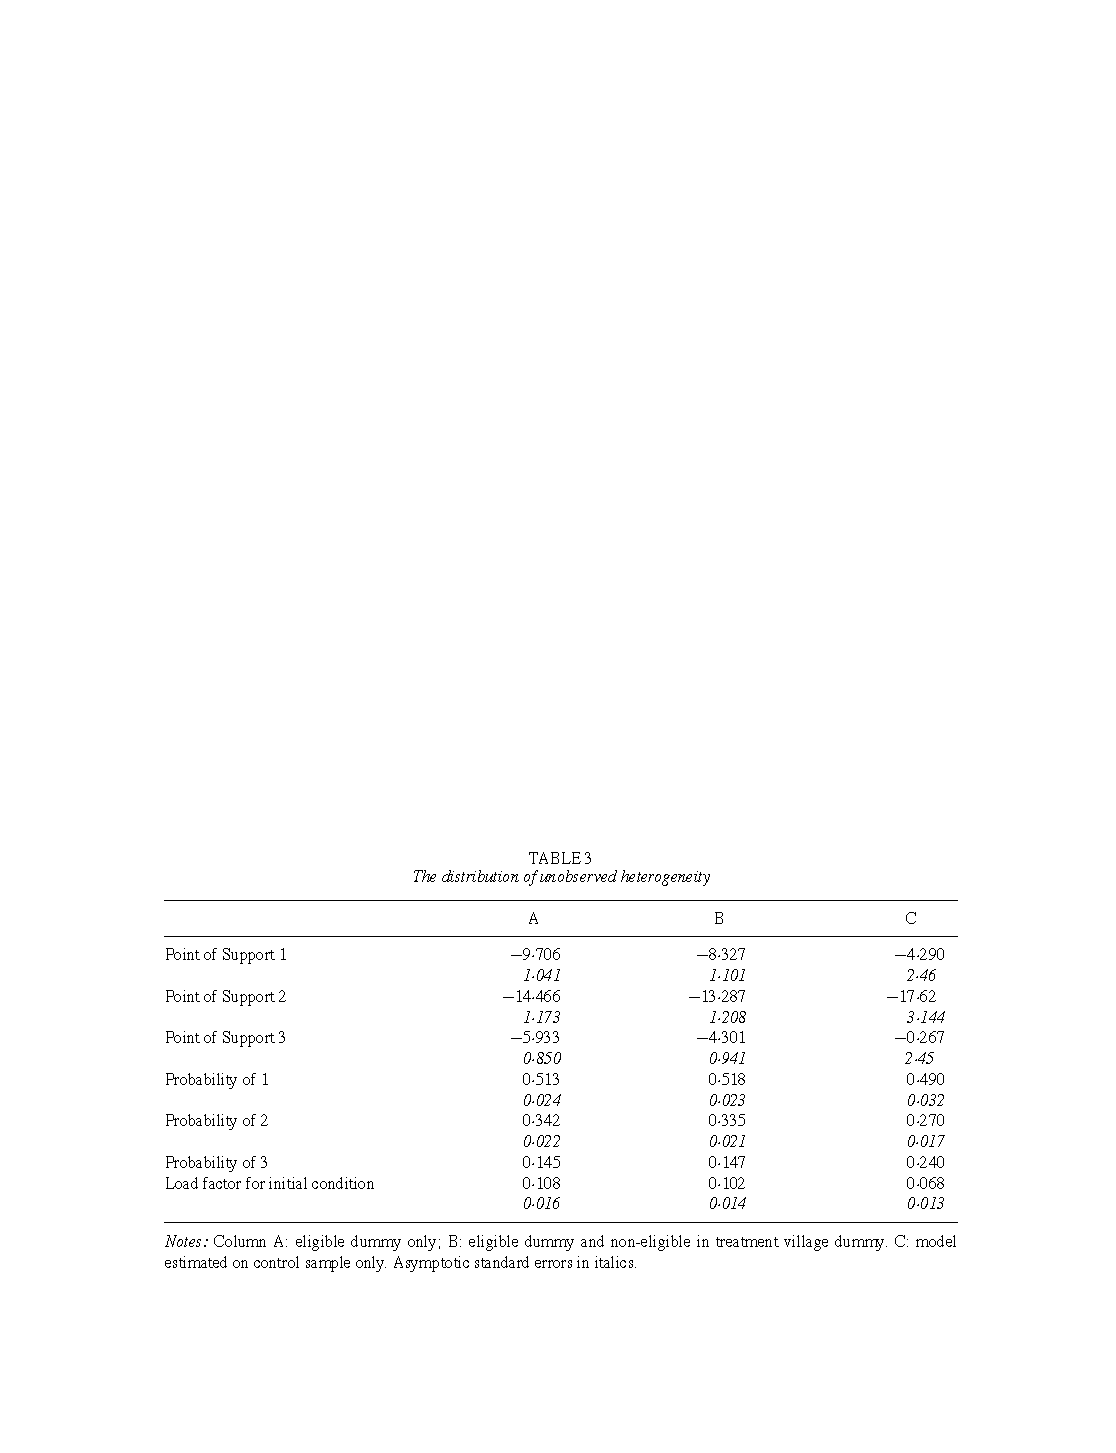
\includegraphics[width=1\linewidth]{image/AttanasioMeghir Santiago2011Figure3.pdf}
\end{figure}

\begin{figure}[H]
\centering
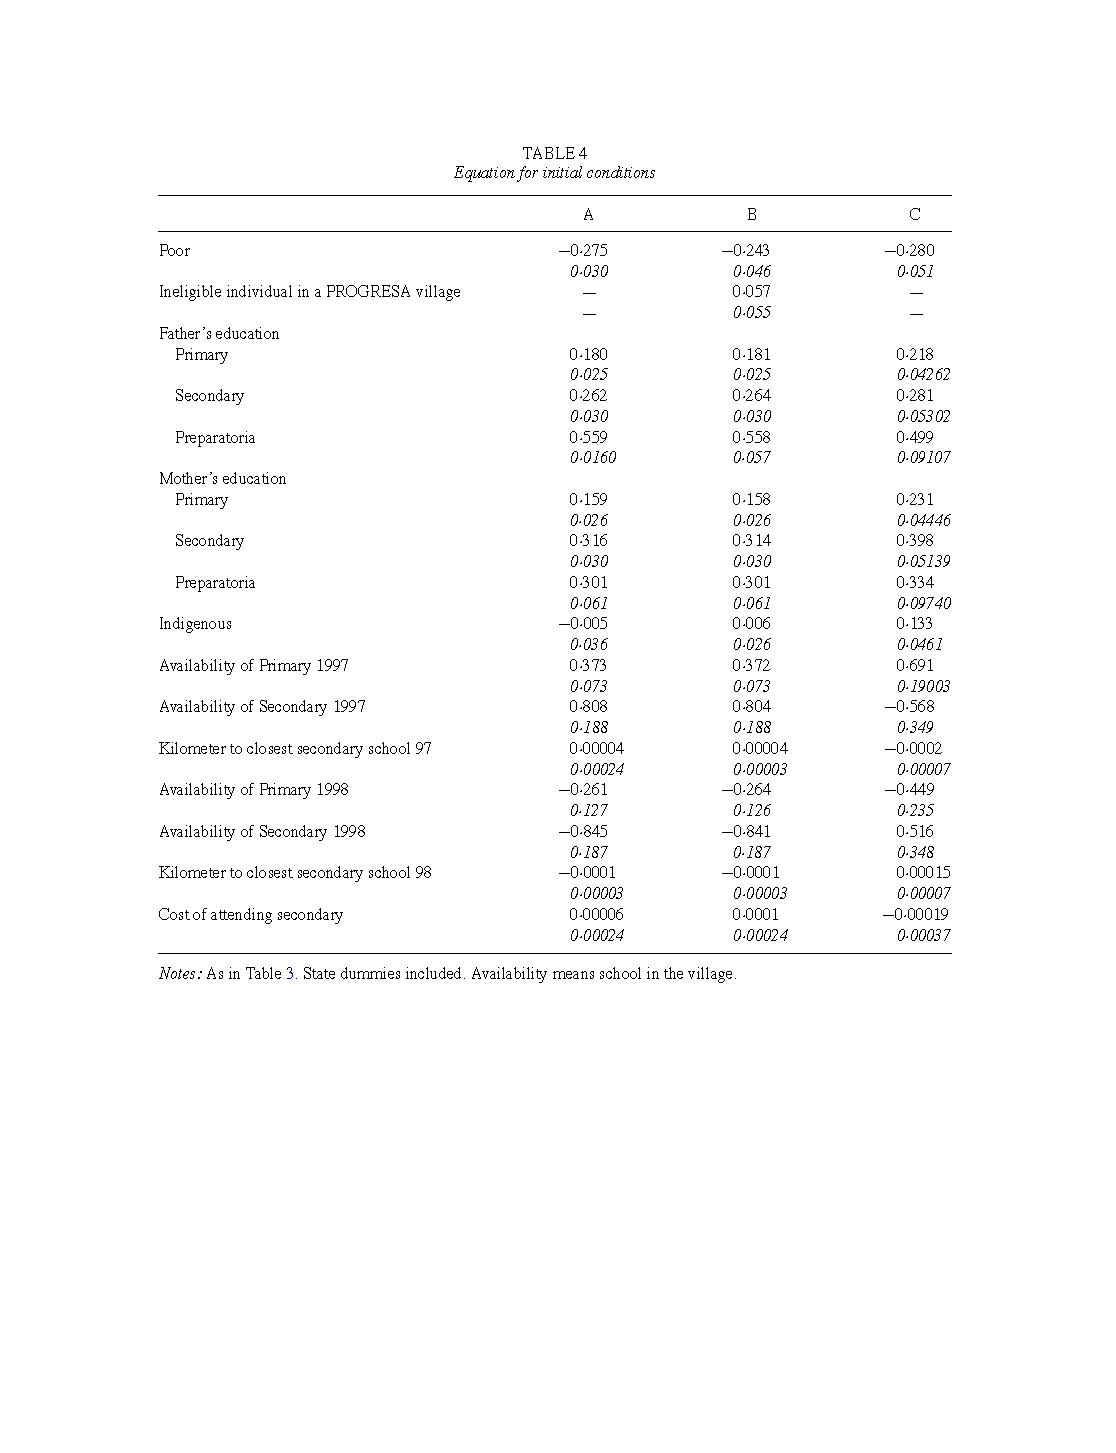
\includegraphics[width=1\linewidth]{image/AttanasioMeghir Santiago2011Figure4.pdf}
\end{figure}
The third column (C) in the tables presents estimates of the model obtained from the control sample only. In this case, the experiment is not used to estimate the model and all incentive effects are captured by the wage, which acts as the opportunity cost of education. The purpose of estimating it is to compare the predictions of a model estimated using the experiment to one that does not and relies on the equality of the the marginal utility of the wage and the grant.

For all specifications, the discount factor was estimated to be between 0.95 and 0.98. This value was obtained from a grid search over several values, for our favourite version of the model.$\footnote{It turns out that approximately the same value of the discount factor maximizes the likelihood function both in Columns 1 and 2 of our tables. The standard errors we report are conditional on the value of the discount factor}$
\begin{figure}[H]
\centering
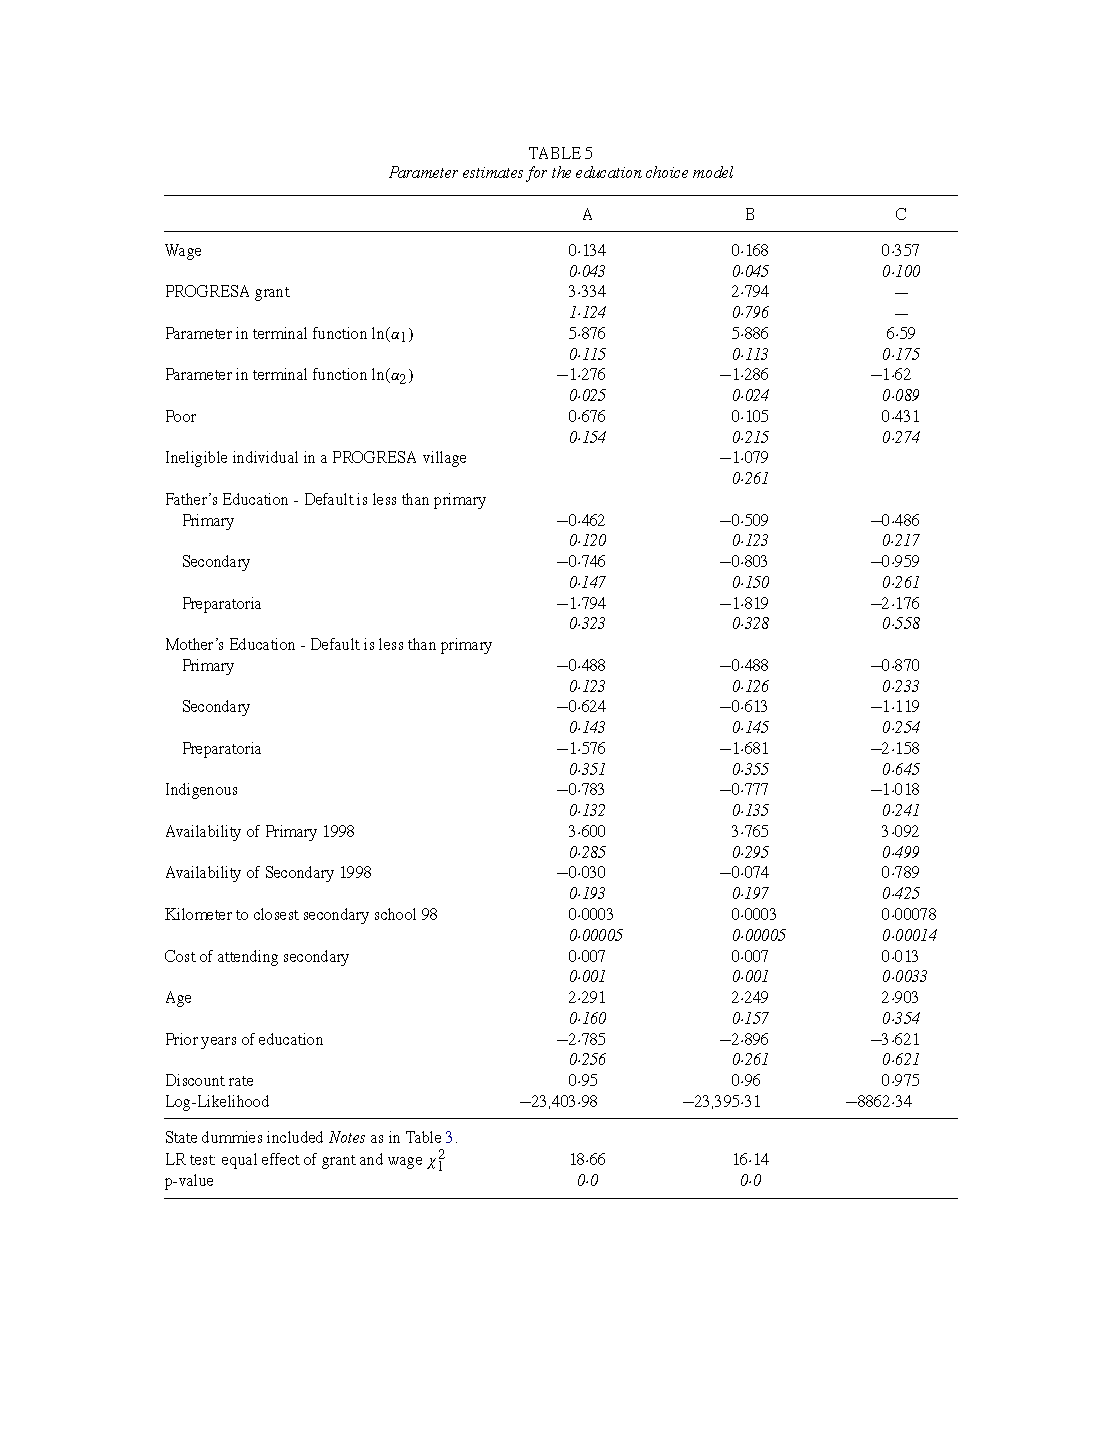
\includegraphics[width=1\linewidth]{image/AttanasioMeghir Santiago2011Figure5.pdf}
\end{figure}
We estimate all the versions of the model on the sample of boys older than 9 and younger than 17. All specifications include, both in the initial condition equation and in the cost of education equation, state dummies, whose estimates are not reported for the sake of brevity. In addition, we have variables reflecting parental education (the excluded groups are heads and spouses with less than completed primary) and parents' ethnicity. We also include the distance from secondary school as well as the cost of attending such school, which in some cases includes fees. Finally, all specifications include a dummy (poor) for programme eligibility (potential if in a control village). This is, effectively, just a measure of wealth.

As mentioned above, we allow for unobserved heterogeneity that is modelled as a discrete variable with three points of support. The same variable enters, with different loading factors, both the utility of going to school equation and the initial condition equations. Such a variable, therefore, plays an important role in that it allows for a flexible specification of unobserved heterogeneity and determines the degree of correlation between the utility of schooling and completed schooling, which, by entering the equation for the current utility of schooling, introduces an important dynamic effect into the model. We therefore start reporting, in Table 3, the estimates of the points of support of the unobserved heterogeneity terms and that of the loading factor of the unobserved heterogeneity terms in the initial condition equation. Three points of support seemed to be enough to capture the heterogeneity in our sample.

We first note that the results do not vary much across the first two specifications, while the estimates in Column $\mathrm{C}$ are a bit different. The estimates in Table 3 reveal that we have three types of children, of which one is very unlikely to go to school and accounts for roughly 15\% of the sample. Given that attendance rates at young ages are above 90\%, it is likely that these are the children that have not been attending primary school and, for some reason, would be very difficult to attract to school. Another group that accounts for about 34\% of the sample is much more likely to be in school. The largest group, accounting for 51\% of the sample, is the middle one. The locations of the points of support for the model that is estimated on the controls only is a bit different, but we can still identify the three groups we have just discussed.

The loading factor for the first two models of the unobserved heterogeneity term is negative as expected. It implies that individuals more likely to have completed a higher level of schooling by 1997 are also more likely to be attending in 1998 due to unobserved factors. Perhaps surprisingly, the loading factor for the third model is positive.

The initial condition $\mathrm{e}\mathrm{d}_{it}$ is modelled, conditional on the unobserved heterogeneity, as an ordered probit with age-specific cut-off points reflecting the fact that different ages will have very different probabilities to have completed a certain grade. Indeed, even the number of cut- off points is age specific, to allow for the fact that relatively young children could not have completed more than a certain grade. To save space, we do not report the estimates of the cut-off points. The discrete random term representing unobserved heterogeneity is added to the normally distributed random variable of the ordered probit, effectively yielding a mixture of normals.

In addition to the variables considered in the specification for school utility, we include among the regressors the presence of a primary and a secondary school and the distance from the nearest secondary school in 1997. It is important to stress that these variables are included in the initial condition model only, in addition to the equivalent variables for 1998, included in both equations. As discussed above, these 1997 variables, which enter the initial condition equation but not the equation for current schooling utility, effectively identify the dynamic effect of schooling on preferences. It is therefore comforting that they are strongly significant, even after controlling for the 1998 variables. This indicates that there is enough variability in the availability of school between 1997 and 1998. Taking all coefficients together it seems that the most discriminating variable is the presence of a primary school in 1997.

The results, which do not vary much across the three columns, also make sense: children living in villages with greater availability of schools in 1997 are better educated, children of better educated parents have, on average, reached higher grades, while children of indigenous households have typically completed fewer grades. Children from poor households have, on average, lower levels of schooling. As for the state dummies, which are not reported, all the six states listed seem to have better education outcomes than Guerrero, one of the poorest states in Mexico, and particularly so Hidalgo and Queretaro.

We now turn to the variables included in the education choice model, reported in the top panel of Table 5. All the variables, except for the grant and the wage, are expressed as determinants of the cost of schooling, so that a positive sign on a given variable decreases the probability of currently attending school. The wage is expressed as a determinant of the utility of work (so given the positive coefficient, an increase in wages decreases school attendance) and the grant is a determinant of the utility of schooling, so that an increase in it increases school attendance. In addition, the coefficient of the grant is expressed as a ratio to the coefficient of the wage, so that a coefficient of 1 indicates that a unitary increase in the grant has the same effect on the utility of school as an increase in the wage has on the utility of work.$\footnote{The wage has been scaled to be interpreted as the earnings corresponding to the period covered by the grant. Thus, the effects are comparable.}$

From a policy perspective, the key parameters of the model are the wage coefficient and the coefficient of the grant itself. An increase in the wage decreases the probability of attending school. On average, the effect of reducing the wage Uy 44\% (which would roughly give a reduction similar to the average grant to beneficiaries) increases the probability of attending school by 2.1\%. This effect cannot Ue inferred directly from the value of the parameter alone and has been obtained from the simulations of the model that we discuss in detail below. The wage effect is higher when we estimate the model on the control villages alone. The difference between the wage coefficient in Columns $\mathrm{B}$ and $\mathrm{C}$ is significant and has a $t$ value of 2.12 based on a Durbin-Wu-Hausman type test.

The value of the grant varies by treatment and control villages (where of course it is zero) and by grade the child could be attending.$\footnote{As mentioned above, in secondary school, the grant is also higher for girls than for boys. However, as we only estimate the model for the latter, we do not exploit this variation.}$ As mentioned above, the coefficient of the grant is expressed as a fraction of the wage coefficient. The values of about 2.8 (or 3.3 for Column A) for this coefficient reported in Table 5 indicates that the effect of the grant on school attendance is considerably larger than the effect of the wage. The hypothesis that the effect of the grant is equal to an equivalent reduction of the wage ($i.e$. that the grant coefficient is one) is strongly rejected by a likelihood ratio test as reported at the bottom of the table.$\footnote{Since this hypothesis relates to a non-linear restriction and subject to a variety of different normalizations the Wald test is not appropriate. See Gregory and Veall (1985).}$ This test rejects the hypothesis that education and consumption can be taken to be separable (in the sense that we explain earlier) and implies the importance of having experimental information to assess the impact of policy in this case.

In terms of background characteristics, belonging to a household with less educated parents leads to lower attendance. This may Ue a reflection of liquidity constraints or different costs of schooling. Perhaps surprisingly, the coefficient of poor (eligible) households is not significantly different from zero once we control for ineligibles in PROGRSA villages, while that on indigenous households indicates that, ceteris paribus, they are more likely to send their children to school. The states that exhibit the higher costs are Queretaro and PueUla, followed by San Luis Potosi and Michoacan, while Veracruz and Guerrero are the cheapest. The costs of attending sec- ondary measured in either distance (since many secondary schools are located in neighbouring village) or in terms of money have a significant and negative effect on attendance.

Both age and grade have a very important effect on the cost of schooling, age increasing and grade decreasing it. The coefficient of age is the way in which the model fits the decline in enrolment rates by age across both treatment and control villages. The effect on the grade captures the dynamics of the model and, as we discussed, is identified by the presence of lagged supply of school infrastructure. We find a very strong effect of state dependence despite the fact that we include age as one of the explanatory variables. The pre-existing level of education is a critical determinant of choice, with increased levels of education having a substantially positive effect on further participation. This is of course an important point since it provides an additional mechanism by which the subsidy may increase educational participation and is likely to be key for simulating alternative policies. It also implies different effects depending on the amount of prior educational participation. The likelihood ratio test for the null that past education does not matter has a $p$ value of zero (the likelihood ratio statistic is 300). Moreover, eliminating habits leads to an overprediction of the program effects.

As we discussed above, we have scant information on the returns to education, so that we include the returns to education among the parameters to be inferred from the differential attendance rates in school. It is therefore important to check what are the returns to education implied by this model. When we compute the return to education implied by the coefficients of the terminal value function, we obtain an estimate of the average return to education of 5\% per year, maybe a bit low in the Mexican context, but above the average return to education observed in our villages.$\footnote{The return is calculated as $r=\displaystyle \frac{\partial\nabla_{T}}{\nabla_{T}\partial ed}$ where $V_{T}=V(ed_{i,18})$ and where the parameters $\alpha_{1}$ and $a_{2}$ are given in their logs in column 3 of Table 5.}$

Cost variables have the expected sign and are significant. For instance, an increase in the distance from the nearest secondary school significantly decreases the probability of attending school. Likewise for an increase in the average cost of attending secondary school. As several of the children in our sample are still attending primary school, we also tried to include variables reflecting the cost and availability of primary schools, but we could not identify any significant effect.


\newpage

\section{SIMULATIONS}
The model is complex and non-linear. To check how the various specifications of the model are able to predict the impact of the grant and to quantify the effect of the main variables of interest from a policy point of view, we present the results of simulations of various versions of the model. We start by comparing the impacts predicted by the different versions of the model with the impacts of PROGRSA as estimated by comparing enrolment rates in treatment and control localities, as we have done in Section 3. We then study changes to the program and alternative policies.

\subsection{Predicting the impact of PROGRESA}
To check how our basic model predicts the impact of the program, we simulate the behaviour of the children in our sample under two different scenarios. The first corresponds to the actual data and includes, in the treatment communities, the grant. It should be stressed that, in these communities, the grant is assumed to be permanent. The second is a scenario in which, counter- factually, we set the grant equal to zero. We then compute the probability of school enrolment of eligible boys in treatment communities under the two scenarios, average these probabilities for different age groups and interpret the difference in probabilities as the impact of the program. When removing (counterfactually) the grant from treatment areas, we compute two predictions. In one case, we keep children wages constant across comparisons, assuming that the pro- gram did not affect wages. This is what one would calculate based on a partial equilibrium model estimated on the controls only. We label this ``effect of Grant--No GE. In a second calculation,

\begin{figure}[H]
\centering
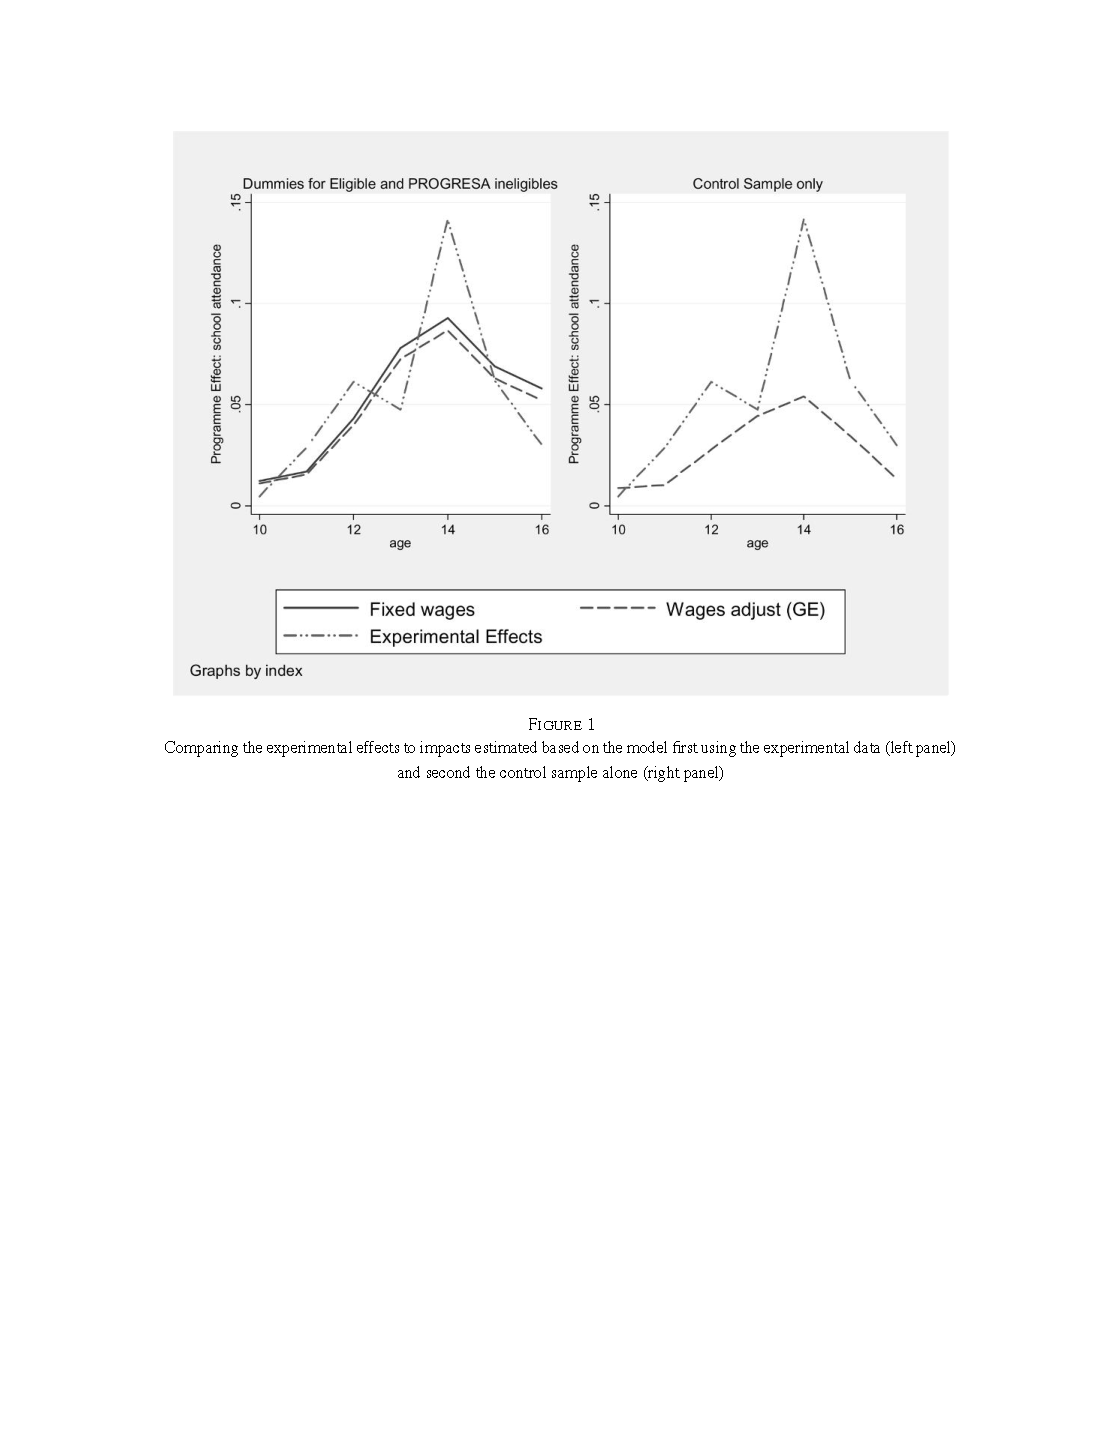
\includegraphics[width=1\linewidth]{image/AttanasioMeghir Santiago2011Figure6.pdf}
\end{figure}

when we remove the grant we also adjust wages downwards based on our estimates of the impact of the grant on wages. We label this ``effect of Grant--GE To these results, plotted in Figure 1, we juxtapose the experimental impacts discussed in Section 3, which is the dotted line.
In Column $\mathrm{C}$ of Tables 3-5, we presented estimates of a model estimated on the sample of control villages only. We have already demonstrated that the effect of the grant is not equivalent to a corresponding reduction of the wage, which is the opportunity cost of education. We interpret this as a rejection of pooling of child and other household income (see estimates in Column $\mathrm{C}$ of the results tables). This in itself implies that a model estimated without the experimental variation cannot accurately predict the effects of the experiment on educational participation. In addition to show how our model predicts the impact of the program, we also want to show the ex- tent to which the rejection of the simpler model that assumes income pooling, is a quantitatively important issue.
The left-hand side panel in Figure 1 relates to our basic model estimated on both the treatment and the control samples. As we plot the difference in probabilities only for eligible children, and as the estimates of most coefficients do not change much between the two versions of the model (with and without the non-eligible treatment village dummies), not surprisingly the age profile of the impacts looks very similar. Therefore, in the figure, we only report one of them.
The right-hand side panel in Figure 1 reports the impacts predicted by the model estimated only on control villages with the income pooling assumption imposed. In this case, the impact of the grant is derived from the coefficient of the wage.

Not surprisingly, the average effect of the treatment (estimated experimentally at 0.05) is predicted quite accurately by the model at $0\cdot 047$. Moreover, the model predicts reasonably well the inverted $\mathrm{U}$-shape of the impact. Estimating the model based on the controls only, we obtain an average effect of $0\cdot 031$. However, what is more interesting is to consider the age pattern of the effect.

Consider first the comparisons that keep wages constant. The age pattern is very similar to the experimental one, except that the model misses the 14\% peak effect at age 14 and compensates with higher effects around these ages. The failure of the model to replicate the peak is unsurprising given the simple and parsimonious functional form we have chosen. On the other hand, when we consider the predictions from the model estimated based on the sample of control villages only, we find that it consistently underestimates the effects of the program by large amounts. This is because the wage effect is much smaller than that of the grant, despite the fact that when we estimate the model on the controls alone we obtain a wage coefficient which is more than twice what we obtain in the sample including the treatment villages.

The experimental evidence, as shown in the wage regression we discussed above, showed that the program pushed up children wages by 6\%. Thus, comparing treatment and control villages does not measure the partial effect of the subsidy on school participation but includes also the effect that the program has through its impact on the labour market in the treatment villages. Thus, the appropriate comparison between experimental effects and model predictions is one that allows for the effect on wages, which is given by the dashed lines in Figure 1. The impact of correcting the effect for wages is minimal in the model estimated on the whole sample. As a result, the model still compares well to the experimental effects. However, when we adjust wages in the model estimated on controls alone, the effect decreases substantially. Noting that this is the most appropriate comparison with the experimental effects, which include the impact on wages, this result shows that the model estimated on the controls alone performs even worse in predicting the experimental results.

The model estimated on the controls only (Column C) differs in a number of ways from that of TW as explained earlier. However, it is interesting to note that it does not perform worse, for the age interval 12-15 than the model TW presented for boys.$\footnote{Todd and Wolpin (2006) estimate the model for boys and girls. For boys aged 12-15 years, they present predicted impacts.}$ It seems to us that using the experimental variation in the grant and not imposing any of the restrictions required for using the controls only is important for understanding how the policy works.

\subsection{Anatomy of PROGRESA and some alternatives}
One of the main advantages of having a structural model is the possibility of performing policy experiments. We now use the model to simulate school participation under different scenarios. First, we compare the effect of the current program with that of a similar program that differs in the way in which the grant varies with the grade attended.
The aim of this exercise is to compare the impact of the current grant, as predicted by our model, to the impact that is obtained when the structure of the grant is changed so as to target the program to those in the most responsive ages. In particular, we focus on a ``balanced budget'' reform of the program. That is, we increase the grant for children above grade 6 and set it to zero for children below that grade. The increase for the older children is calibrated so that, taking into account the response of children schooling choices to the change, the overall cost of the program is left unchanged (at least for our sample).
\begin{figure}[H]
\centering
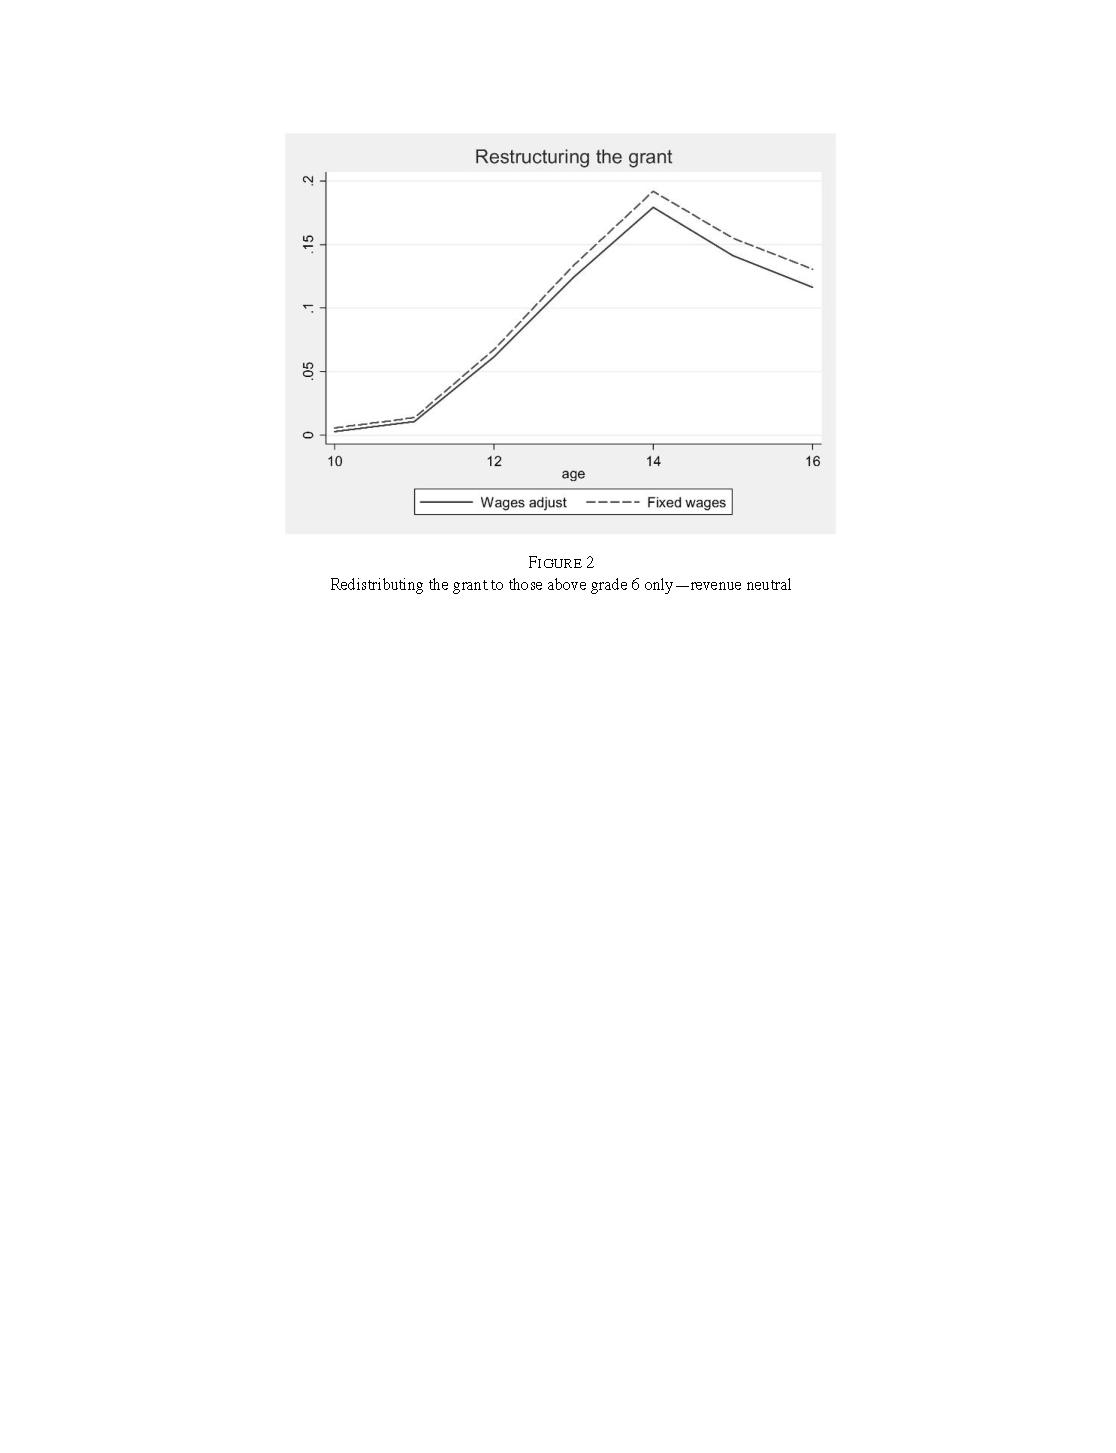
\includegraphics[width=0.75\linewidth]{image/AttanasioMeghir Santiago2011Figure7.pdf}
\end{figure}

We plot the result of this exercise in Figure 2, where we again show the results with no wage adjustment (continuous line) and with a GE adjustment. Performing the GE adjustment is now a bit more complicated than in the previous exercise. The amount by which children wages would change with the counterfactual grant structure has to be extrapolated. We do that by using the elasticities discussed in Section 4.5.

The graph shows that by targeting the grant to the older children we can almost double the impact relative to the predicted effect from the model shown in the left panel of Figure 1. This occurs with no effect on the school participation of the younger primary age children. This is not surprising since the grant hardly changes their behaviour in the first place because almost all children go to school below grade 6, making it an unconditional transfer for that age group. The overall resources targeted to families with children do not change with this reform, but the incentive structure does.
This change to the grant structure seems to suggest a modification to the program that would much improve its ability to increase enrolment rates. This is particularly important because the modified program costs, in the steady state, the same amount as the current one. From the point of view of the households, note that they receive the same amount of resources over time: what changes is when they receive them. If households can borrow against the future grant, then the only effect of this reform is to improve incentives for school participation at later ages. If, on the other hand, families are liquidity constrained, the trade-off may be more serious, particularly if the grant at a younger age affects nutrition or other child inputs.$\footnote{Attanasio and Kaufmann (2009) show that for the Oportunidades/PROGRESA population, liquidity constraints can be important.}$ Attanasio and RuUio-Codina (2008) show that the impact of the PROGRSA grant on a variety of nutritional outcomes for very young children does not depend on whether they have primary school age siblings. This indicates that a change in the grant structure such as the one simulated here may not have large negative side-effects. More recently, the Mexican government is piloting two versions of the program in which primary school grants are eliminated and secondary school grants are increased.
\begin{figure}[H]
\centering
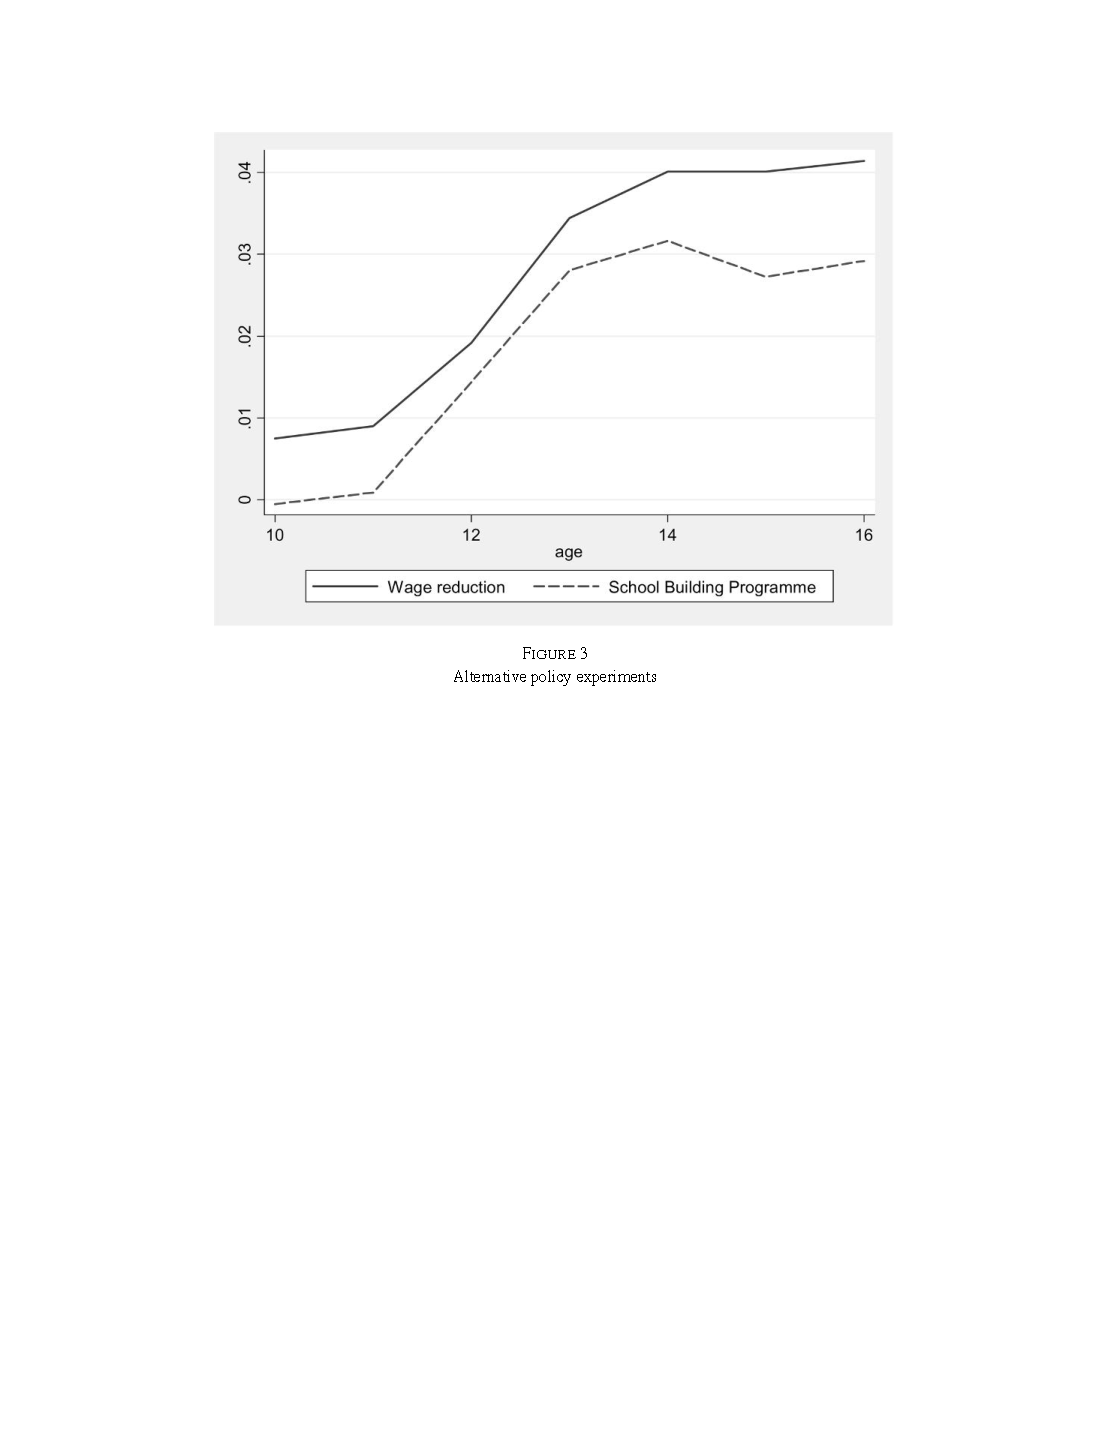
\includegraphics[width=0.75\linewidth]{image/AttanasioMeghir Santiago2011Figure8.pdf}
\end{figure}
We next consider two alternative experiments. In particular, we consider the effect of decreasing the wage by an amount equivalent to the grant and the effect of reducing the distance to school to a maximum of 3 $\mathrm{k}\mathrm{m}\mathrm{s}$. All three experiments are summarized in Figure 3. In all cases, we use the model $\mathrm{B}$ in the tables. No grant is our baseline.

First, we decrease the wage by an amount equivalent to the grant.$\footnote{The reduction is proportional so as to give an average amount equivalent to the grant. The grant, however, is additive. So we would not expect the effects of the wage to be distributed equally because the wage varies with age much more steeply than the grant.}$ We see that the effect of the wage is estimated to be much lower than the grant; for example at age 15 the incentive effect is less than half the one in Figure 1. This evidence re-emphasizes the point already made, that the experimental data provides information on behaviour that may not be available through standard observational data.
In the next experiment, we demonstrate the effects of a potential school building program that would reduce the distance of secondary schools to no more than 3 km. We consider this because it could constitute an alternative policy to subsidizing participation (although we do not claim that this policy is equivalent in terms of cost or in terms of other benefits such as better nutrition and its impact). According to our parameter estimates, the effect is modest as it would increase participation by just about 3 percentage points at age 15.

\newpage

\section{CONCLUSIONS}
In this paper, we demonstrate the power of using an economic model to analyse data from a major social experiment, namely PROGRSA in Mexico. Conversely, we also show the usefulness of using experimental data to estimate a structural economic model. The welfare program we consider was originally applied to rural Mexico and aimed, among other things, at increasing school enrolment rates among poor children.

We start by showing some of the effects of this program on school participation. As the pro- gram was randomized across villages, inducing truly exogenous variation in the incentives to attend school, by offering a subsidy for attendance, estimation of its impact is relatively straight- forward. After presenting some evidence based on simple treatment/control comparisons, we argue that many questions are left unanswered by this type of techniques and propose the use of a structural model.

By interpreting the data through the viewpoint of a dynamic model, one can investigate how the impacts of the program would be different if one were to change some of its parameters. In particular, we analyse what would happen to the program's impact on enrolment by changing the structure of the grants with age. This type of analysis is instrumental to the design of effective interventions and cannot be performed without a well-specified behavioural model. We can also compare the impacts of the program with alternative policies, such as a program that would reduce the distance of the households in our sample from the nearest secondary school. Therefore, we show that only through this kind of modelling approach is it possible to answer questions that are more general than the specific focus of the evaluation.

But this is not a one way street: we also argue that the use of the experimental data and the genuine exogenous variation it induces allows us to identify models that are richer than those that could be identified based on standard observational data. In our specific context, we show that, although the program operates by changing the relative price of education and its opportunity cost, the economic incentives it provides are much larger than those provided by changes in children wages. This is important not only from a policy point of view but also for modelling if one notes that without the experimental variation our model could not be estimated. Our approach provides a rich set of results and at the same time points to the importance of the interaction between economic models and social experiments for the purposes of evaluation and understanding behaviour.

The experimental design of the evaluation data, where the program was randomized across communities, and the fact that the localities in the sample are relatively isolated allow one to estimate the GE effect that the program has on children wages. Having estimated these effects, we incorporate this additional channel in our structural model, both at the estimation stage (where our estimated wage equation incorporates the GE effects) and in performing the simulation of alternative interventions.

The model we estimate fits the data well and predicts impacts that match the results obtained by the experimental evaluation closely. They indicate that the program is quite effective in increasing the enrolment of children at the end of their primary education, a fact that has been noticed in several evaluations of conditional cash transfers in Latin America. On the other hand, the program does not have a big impact on children of primary school age, partly because enrolment rates for these children are already quite high.

We identify relatively large GE effects of the program on child wages: in the treatment localities, child wages are about 6\% higher than in control localities. Remarkably, this fact had not been noticed in the large empirical literature on PROGRSA. Although these effects and the impact that the program is observed to have on school enrolment (and child labour supply) imply relatively large elasticities of wages to changes in enrolment, the attenuating effect on the impact of the grant is not large.

The heterogeneity of the program impacts by age has suggested the possibility of changing the structure of the grant, reducing or eliminating the primary school grant and increasing the size of the grant for secondary school. This proposal, that has been considered in urban Mexico and in Columbia, can be analysed with the help of our structural model. The simulations we perform indicate that the effect on school participation could be much improved by offering more resources to older children and less to relatively younger one. By taking into account behavioural responses, we simulate changes to the program that result in the same amount of resources spent by the program and yet obtain much larger impacts on school enrolment of older children.

Some words of caution are obviously in order when considering the results of our simulations. It should be pointed out, for instance, that our model is silent as to the effect of the grant on other dimensions of child development. Since most young children go to school anyway, the grant for them is effectively unconditional and can have other effect such as on their nutrition and resulting physical and cognitive development. Although the reformulated grant could trans- fer the same resources to the families whose children continued school attendance, albeit with different timing the effects on these other dimensions we do not model could be different in the presence of liquidity constraints; moreover, fewer resources would end up with those who despite the increased grant drop out of school anyway. Nevertheless,our results imply that in terms of school participation, changing the age structure of the grant would achieve different results.

\newpage

\section*{APPENDIX}
{\it Difference in difference estimates of PROGRESA impacts}

In Table Al, we report the estimated impacts of PROGRESA on boy's enrolment for each age from 10 to 16, as well as the average impact for boys aged 10-16 years and for the age group 12-15. The sample we use in the estimation of the structural model and for Table 2 is slightly different because of attrition. To compute the estimates in Table Al, we use a slightly different sample because of the necessity to use baseline data.
\begin{figure}[H]
\centering
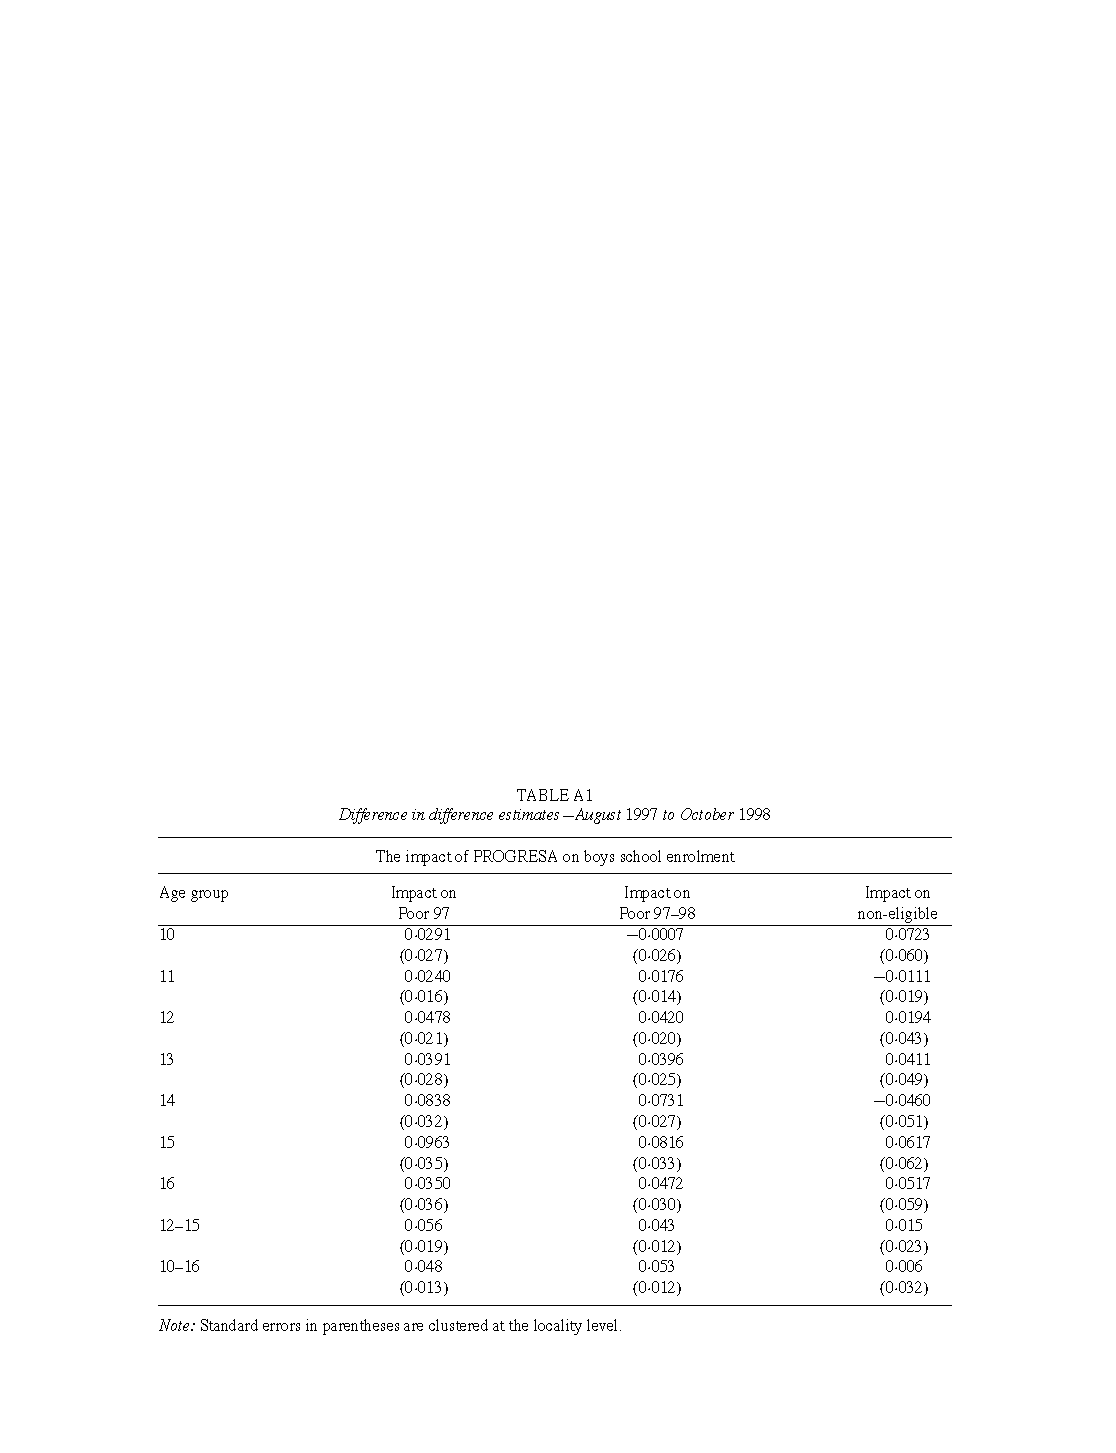
\includegraphics[width=0.75\linewidth]{image/AttanasioMeghir Santiago2011Figure9.pdf}
\end{figure}

\subsection*{Supplementary Data}
Supplementary data are available at {\it Review of Economic Studies} online.







































\newpage
\section*{References}
ANGELUCCI, M. and DEGIORGI, G. (2009), ``Indirect Effects of an Aid Program: The Case of Progresa and Consumption {\it American Economic Review}, 99, 486-508.

ATTANASIO, O. and RUBIO-CODINA, M. (2008), ${\rm Re}$-evaluating Conditional Cash Transfers: Is the Oportunidades Primary School Stipend Necessary?'' (Mimeo, $\mathrm{I}\Gamma \mathrm{S}$).

ATTANASIO, O. $\mathrm{P}$ and KAUFMANN, K. M. (2009) ``Educational Choices, Subjective Expectations, and Credit Constraints'' (NBER Working Paper No. 15087, National Bureau of Economic Research).

BEHRMAN, J. (1999), ``Education, Health and Demography in Latin America Around the End of the Century: What Do We Know? What Questions Should Be Explored?'' (Mimeo, IADB).

BEHRMAN, J., DURYEA, S. and SZ\'{E}KELY, M. (1999), ``Schooling Investments and Aggregate Conditions: A House- hold Survey-Based Approach for Latin America and the CariuUean'' (OCE Working Paper No. 407, IADB, Washing- ton; http: $//\mathrm{w}\mathrm{w}\mathrm{w}$ iadb.$\mathrm{o}\mathrm{r}\mathrm{g}/\mathrm{r}\mathrm{e}\mathrm{s}/\mathrm{p}\mathrm{u}\mathrm{b}\mathrm{l}\mathrm{i}\mathrm{c}\mathrm{a}\mathrm{t}\mathrm{i}\mathrm{o}\mathrm{n}\mathrm{s}/\mathrm{p}\mathrm{u}\mathrm{b}\mathrm{f}\mathrm{i}\mathrm{l}\mathrm{e}\mathrm{s}/\mathrm{p}\mathrm{u}\mathrm{b}\mathrm{W}\mathrm{P}-407$ pdf).

BEHRMAN, J., DURYEA, S. and SZ\'{E}KELY, M. (2000), ``Households and Economic Growth in Latin America and the CariuUean'' (Mimeo, GDN).

BEHRMAN, J. and TODD, $\mathrm{P}$ (1999), ``Randomness in the Experimental Samples of PROGRESA (Education, Health, and Nutrition Program (IFPRI; http: $//\mathrm{w}\mathrm{w}\mathrm{w}$ ifpri. $\mathrm{o}\mathrm{r}\mathrm{g}/\mathrm{t}\mathrm{h}\mathrm{e}\mathrm{m}\mathrm{e}\mathrm{s}/\mathrm{P}\mathrm{R}\mathrm{O}\mathrm{G}\mathrm{R}\mathrm{S}\mathrm{A}/\mathrm{p}\mathrm{d}\mathrm{f}/\mathrm{B}\mathrm{e}\mathrm{h}\mathrm{r}\mathrm{m}\mathrm{a}\mathrm{n}\mathrm{T}\mathrm{o}\mathrm{d}\mathrm{d}_{-}$random.$\mathrm{p}\mathrm{d}\mathrm{f}.$
BLUNDELL, R., CHIAPPORI, $\mathrm{P}$ A. and MEGHIR, C. (2005), ``Collective Labour Supply with Children {\it Journal of Political Economy}, 113, 1277-1306.

BLUNDELL, R., CHIAPPORI, $\mathrm{P}$ A., MAGNAC, T. and MEGHIR, C. (2007), ``Collective LaUour Supply: Heterogeneity and Non-participation'', {\it Review of Economic Studies}, 74, $417A45.$
BROWNING, M. and MEGHIR, C. (1991), ``The Effects of Male and Female Labor Supply on Commodity Demands {\it Econometrica}, 59, 925-951.

BURTLESS, G. and HAUSMAN, J. A. (1978), ``The Effect of Taxation on Labor Supply: Evaluating the Gary Negative Income Tax Experiment {\it Journal of Political Economy}, 86, 1103-1130.

CAMERON, S. V and HECKMAN, J. J. (1998), ``Life Cycle Schooling and Dynamic Selection Bias: Models and Evidence for Five Cohorts of American Males {\it Journal of Political Economy}, 106, 262-333.

CUNHA, $\Gamma.$, HECKMAN, J. J. and NAVARRO, S. (2007), ``The Identification and Economic Content ofOrdered Choice Models with Stochastic Thresholds {\it International Economic Review}, 48.

DEARDEN, L., EMMERSON, $\mathrm{C}$ , FRAYNE, C. and MEGHIR, C. (2009), ``Conditional Cash Transfers and School Dropout Rates {\it Journal of Human Resources}, 44, 827-857.

GREGORY, A. $\mathrm{W}$ and VEALL, M. R. (1985), ``Formulating Wald Tests of Nonlinear Restrictions {\it Econometrica}, 54, 1465-1468.

HECKMAN, J. J. (1979), ``Sample Selection Bias as a Specification Error {\it Econometrica}, 153-161.

HECKMAN, J. J. and SINGER, B. (1984), ``A Method for Minimizing the Impact of Distributional Assumptions in Econometric Models for Duration Data {\it Econometrica}, 52, 271-320.
IFPRI, (2002), ``M\'{e}xico- PROGRESA rompiendo el ciclo de la poUreza $\mathrm{h}\mathrm{t}l\mathrm{p}://\mathrm{w}\mathrm{w}\mathrm{w}\mathrm{i}$fpri.$\mathrm{o}\mathrm{r}\mathrm{g}/\mathrm{n}\mathrm{o}\mathrm{d}\mathrm{e}/2440.$

MEGHIR, C. and PISTAFERRI, L. (2004), ``Income Variance Dynamics and Heterogeneity {\it Econometrica}, 1-32.

MOFFITT, R. A. (1979), ``The Labor Supply Response in the Gary Experiment {\it Journal of Human Resources}, 14, $477A87.$

ORCUTT, G. H. and ORCUTT, A. G. (1968), ``Incentive and Disincentive Experimentation for Income Maintenance Policy Purposes {\it American Economic Review}, 58, 754-772.

RAWLINGS, L. (2004), ``A New Approach to Social Assistance: Latin America's Experience with Conditional Cash Transfer Programs'' (World Bank Social Protection Discussion Paper No. 0416).

SCHULTZ, $\mathrm{T} \mathrm{P}$ (2004), ``School Subsidies for the Poor: Evaluating the Mexican Progresa Poverty Program {\it Journal of Development Economics},74, 199-250.

SKOUFIAS, E. (2001), ``PROGRESA and Its Impacts on the Human Capital and Welfare of Households in Rural Mexico: A Synthesis of the Results of an Evaluation by IFPRI'' (IFPRI; http: $//\mathrm{w}\mathrm{w}\mathrm{w}\mathrm{i}$fpri.$\mathrm{o}\mathrm{r}\mathrm{g}/\mathrm{t}\mathrm{h}\mathrm{e}\mathrm{m}\mathrm{e}\mathrm{s}/\mathrm{P}\mathrm{R}\mathrm{O}\mathrm{G}\mathbb{R}\mathrm{S}\mathrm{A}/ \mathrm{p}\mathrm{d}\mathrm{f}/\mathrm{S}\mathrm{k}\mathrm{o}\mathrm{u}\mathrm{f}\mathrm{i}\mathrm{a}\mathrm{s}_{-}$finalsyn. pdf).

THOMAS, D. (1990), ``Intra-Household Resource Allocation: An Inferential Approach {\it Journal of Human Resources}, 25, 635-664.

TODD, $\mathrm{P}$ and WOLPIN, K. (2006), ``Using Experimental Data to Validate a Dynamic Behavioral Model of Child Schooling and Fertility: Assessing the Impact of a School Subsidy Program in Mexico {\it American Economic Review}, 96, 1384-1417.
\end{document}